\documentclass[ALICE,manyauthors]{cernphprep}

\usepackage[comma,square,numbers,sort&compress]{natbib}
\usepackage{hyperref}
\usepackage{lineno}
%\usepackage{subcaption}
\usepackage{subfigure}
\usepackage{tikz}
\usepackage[section]{placeins}
\usepackage {multicol}% Multi column in the table
\usepackage {multirow}% Multi row in the table
\usepackage {units}
\usepackage {array}
\usepackage{verbatim}
\usepackage{dblfloatfix} % for fixing tables at certain places of the page

%\usepackage[dvipsnames]{xcolor}
\linenumbers

% $Id: commands.tex 934 2013-06-19 20:56:45Z mfloris $

\newcommand{\mrm}[1]{\mathrm{#1}}
\newcommand{\mrmo}[1]{\mathrm{\overline{#1}}}
\newcommand{\bsb}[1]{\boldsymbol{#1}}
\newcommand{\circit}{\item[$\circ$]}

\newcommand{\ITS}          {\rm{ITS}}
\newcommand{\TOF}          {\rm{TOF}}
\newcommand{\ZDC}          {\rm{ZDC}}
\newcommand{\ZDCs}         {\rm{ZDCs}}
\newcommand{\ZNA}          {\rm{ZNA}}
\newcommand{\ZNC}          {\rm{ZNC}}
\newcommand{\SPD}          {\rm{SPD}}
\newcommand{\SDD}          {\rm{SDD}}
\newcommand{\SSD}          {\rm{SSD}}
\newcommand{\TPC}          {\rm{TPC}}
\newcommand{\VZERO}        {\rm{VZERO}}
\newcommand{\VZEROA}       {\rm{VZERO-A}}
\newcommand{\VZEROC}       {\rm{VZERO-C}}
\newcommand{\pip}          {$\pi^{+}$}
\newcommand{\pim}          {$\pi^{-}$}
\newcommand{\kap}          {K$^{+}$}
\newcommand{\kam}          {K$^{-}$}
\newcommand{\pbar}         {$\rm\overline{p}$}
\newcommand{\kzero}        {\ensuremath{{\rm K}^{0}_{S}}}
\newcommand{\kstar}        {\ensuremath{{\rm K}^{*}}}
\newcommand{\He}           {\ensuremath{^{3}{\rm He}}}
\newcommand{\LH}           {\ensuremath{^{3}_{\Lambda}{\rm H}}}
\newcommand{\vzero}        {\ensuremath{{\rm V}^0}}
\newcommand{\lmb}          {\ensuremath{\Lambda}}
\newcommand{\almb}         {\ensuremath{\bar{\Lambda}}}
\newcommand{\allpart}      {$\pi^{\pm}$, K$^{\pm}$, \kzero, p(\pbar) and \lmb(\almb)}
\newcommand{\allpi}        {$\pi^{\pm}$}
\newcommand{\allk}         {K$^{\pm}$}
\newcommand{\allp}         {p(\pbar)}
\newcommand{\alllmb}       {\lmb(\almb)}
\newcommand{\degree}       {$^{\rm o}$}
\newcommand{\dg}           {\mbox{$^\circ$}}
\newcommand{\dedx}         {\ensuremath{\mathrm{d}E/\mathrm{d}x}}
\newcommand{\dndy}         {d$N$/d$y$}
\newcommand {\ee}            {\mbox{e$^+$e$^-$}}
\newcommand{\pp}           {pp}
\newcommand{\ppbar}        {\mbox{$\mathrm {p\overline{p}}$}}
\newcommand{\PbPb}         {\mbox{Pb--Pb}}
\newcommand{\pPb}          {\mbox{p--Pb}}
\newcommand{\AuAu}         {\mbox{Au--Au}}
\newcommand{\pseudorap}    {\mbox{$\left | \eta \right | $}}
\newcommand{\dNdeta}       {\ensuremath{\mathrm{d}N_\mathrm{ch}/\mathrm{d}\eta}}
\newcommand{\dNdy}         {\ensuremath{\mathrm{d}N/\mathrm{d}y}}
\newcommand{\dNdptdy}      {\ensuremath{\mathrm{d}N/{\rm d}\pt\mathrm{d}y}}
\newcommand{\dNdyst}       {\ensuremath{\sqrt{\frac{dN_\pi/dy}{s_T}}}}
\newcommand{\dNdetatr}     {\mathrm{d}N_\mathrm{tracklets}/\mathrm{d}\eta}
\newcommand{\dNdetar}[1]   {\mathrm{d}N_\mathrm{ch}/\mathrm{d}\eta\left.\right|_{|\eta|<#1}}
\newcommand{\lum}          {\, \mbox{${\rm cm}^{-2} {\rm s}^{-1}$}}
\newcommand{\barn}         {\, \mbox{${\rm barn}$}}
\newcommand{\m}            {\, \mbox{${\rm m}$}}
\newcommand{\ncls}         {\ensuremath{N_{cls}}}
\newcommand{\nsigma}       {\ensuremath{n\sigma}}
\newcommand{\dcaxy}        {\ensuremath{{\rm DCA}_{xy}}}
\newcommand{\dcaz}         {\ensuremath{{\rm DCA}_{z}}}
\newcommand{\EcrossB}      {E$\times$B}%{\ensuremath{{\rm E}\times{\rm B}}}
\newcommand{\bb}           {Bethe-Bloch}
\newcommand{\s}            {\ensuremath{\sqrt{s}}}
\newcommand{\pt}           {\ensuremath{p_\mathrm{T}}}
\newcommand{\pT}           {\ensuremath{p_{\rm T}}}
\newcommand{\hlab}         {\ensuremath{\eta_{\rm lab}}}
\newcommand{\ynn}         {\ensuremath{y_{\rm NN}}}
\newcommand{\ycms}         {\ensuremath{y_{\rm CMS}}}
\newcommand{\ylab}         {\ensuremath{y_{\rm lab}}}
\newcommand{\ppi}          {\ensuremath{{\rm p}/\pi}}
\newcommand{\kpi}          {\ensuremath{{\rm K}/\pi}}
\newcommand{\lpi}          {\ensuremath{{\rm \Lambda}/\pi}}
%\newcommand{\ppi}          {\ensuremath{(\pi^+ + \pi^-)/({\rm K}^+ + {\rm K}^-)}}
%\newcommand{\kpi}          {\ensuremath{({\rm p} + {\rm \bar p})/({\rm K}^+ + {\rm K}^-)}}
\newcommand{\mt}           {\ensuremath{m_{\rm T}}}
\newcommand{\snn}          {\ensuremath{\sqrt{s_{\rm NN}}}}
\newcommand{\snnbf}        {\ensuremath{\mathbf{{\sqrt{s_{\mathbf NN}}}}}}
\newcommand{\sonly}        {\ensuremath{\sqrt{s}}}
\newcommand{\Npart}        {\ensuremath{N_\mathrm{part}}}
\newcommand{\avNpart}      {\ensuremath{\langle N_\mathrm{part} \rangle}}
\newcommand{\avNpartdata}  {\ensuremath{\langle N_\mathrm{part}^{\rm data} \rangle}}
\newcommand{\Ncoll}        {\ensuremath{N_\mathrm{coll}}}
\newcommand{\Dnpart}       {\ensuremath{D\left(\Npart\right)}}
\newcommand{\DnpartExp}    {\ensuremath{D_{\rm exp}\left(\Npart\right)}}
\newcommand{\dNdetapt}     {\ensuremath{\dNdeta\,/\left(0.5\Npart\right)}}
\newcommand{\dNdetaptr}[1] {\ensuremath{\dNdetar{#1}\,/\left(0.5\Npart\right)}}
\newcommand{\dNdetape}     {\left(\ensuremath{\dNdeta\right)/\left(\avNpart/2\right)}}
\newcommand{\dNdetaper}[1] {\ensuremath{\dNdetar{#1}\,/\left(\avNpart/2\right)}}
\newcommand{\dndydpt}      {\ensuremath{{\rm d}^2N/({\rm d}y {\rm d}p_{\rm t})}}
\newcommand{\abs}[1]       {\ensuremath{\left|#1\right|}}
\newcommand{\signn}        {\ensuremath{\sigma^{\rm inel.}_{\rm NN}}}
\newcommand{\vz}           {\ensuremath{V_{z}}}
\newcommand{\Tfo}          {\ensuremath{{T}_{\rm kin}}}
\newcommand{\Tch}          {\ensuremath{{T}_{\rm ch}}}
\newcommand{\bT}           {\ensuremath{\beta_{\rm T}}}
\newcommand{\avbT}         {\ensuremath{\left< \beta_{\rm T}\right>}}
\newcommand{\avpT}         {\ensuremath{\left< \pt \right>}}
\newcommand{\muB}          {\ensuremath{\mu_{B}}}
\newcommand{\stat}         {({\it stat.})}
\newcommand{\syst}         {({\it sys.})}
\newcommand{\Fig}[1]       {Fig.~\ref{#1}}
\newcommand{\Figure}[1]    {Figure~\ref{#1}}
%\newcommand{\Ref}[1]       {Ref.~\cite{#1}}
%\newcommand{\green}[1]     {\textcolor{green}{#1}}
%\newcommand{\blue}[1]      {\textcolor{blue}{#1}}
%\newcommand{\red}[1]       {\textcolor{red}{#1}}
%\newcommand{\white}[1]     {\textcolor{white}{#1}}
\newcommand{\gevc}         {\ensuremath{{\rm GeV}/c}}
\newcommand{\mevc}         {\ensuremath{{\rm MeV}/c}}
\newcommand{\gs}           {\ensuremath{\gamma_{s}}}
\newcommand{\gq}           {\ensuremath{\gamma_{q}}}
\newcommand{\gc}           {\ensuremath{\gamma_{c}}}
\newcommand{\chindf}       {\ensuremath{\chi^{2}/{\rm NDF}}}
\newcommand{\avg}[1]       {\ensuremath{\left\langle#1\right\rangle}}
\newcommand{\etalab}       {\ensuremath{\eta_{{\rm lab}}}}
\newcommand {\gammas}			{\ensuremath{\gamma_{\mathrm{s}}}}

\newcommand{\DNDETAINEL}{5.31~$\pm$~0.18\xspace}
\newcommand{\DNDETAINELGTZERO}{6.46~$\pm$~0.19\xspace}
\newcommand{\DNDETAINELGTZEROONE}{6.61~$\pm$~0.20\xspace}

\newcommand{\inelgtzero}{INEL$>$0\xspace}
\newcommand{\average}[1]{\ensuremath{\langle #1 \rangle}\xspace}
\newcommand{\mpt}        {\ensuremath{\langle\pt\rangle}\xspace}
\newcommand{\nch}        {\ensuremath{N_\mathrm{ch}}\xspace}
\newcommand{\mnch}      {\ensuremath{\langle\nch\rangle}\xspace}
\newcommand{\nchacc}        {\ensuremath{N_\mathrm{ch}^\mathrm{acc}}\xspace}
\newcommand{\mnchacc}      {\ensuremath{\langle\nchacc\rangle}\xspace}
\newcommand{\inelg}     {\ensuremath{\mathrm{INEL}_{>0}}}



\newcommand{\dndeta}{\ensuremath{{\rm d}N_{\rm ch}/{\rm d}\eta}\xspace}
\newcommand{\dndpt}{\ensuremath{{\rm d}N_{\rm ch}/{\rm d}\pt}\xspace}
\newcommand{\etaless}[1]{\ensuremath{\left|\eta\right| < #1}\xspace}
\newcommand{\dndetaless}[1]{\ensuremath{{\rm d}N_{\rm ch}/{\rm d}\eta|_{\etaless{#1}}}\xspace}
\newcommand{\avdndeta}{\ensuremath{\langle \dndeta \rangle}}
\newcommand{\zvtx}{\ensuremath{z_\mathrm{vtx}}}
\newcommand{\pythiae}{\ensuremath{\mathrm{PYTHIA}\,8}}
%\newcommand{\pythiam}{\ensuremath{\mathrm{PYTHIA}\,8\,\mathrm{Monash}\,2013}}
\newcommand{\pythiam}{\ensuremath{\mathrm{PYTHIA}\,8\,\mathrm{Tune\,4C}}}
\newcommand{\pythiashoving}{{\ensuremath{\mathrm{PYTHIA}\,8~\mathrm{String}~}}\ensuremath{\mathrm{Shoving}}}
\newcommand{\epos}{{\ensuremath{\mathrm{EPOS}\,~\mathrm{LHC}}}}
%\newcommand{\pythiashoving}{\ensuremath{\mathrm{PYTHIA}\,8~\mathrm{String}~}\linenomath{-}\ensuremath{\mathrm{Shoving}}}
\newcommand{\pttrig}{\ensuremath{p_\mathrm{T,\,trig}}}
\newcommand{\ptassoc}{\ensuremath{p_\mathrm{T,\,assoc}}}
\newcommand{\ptjet}{\ensuremath{p_\mathrm{T,\,jet}^\mathrm{ch}}}
\newcommand{\ptlead}{\ensuremath{p_\mathrm{T,\,LP}}}
\newcommand{\pttrigassoc}{\ensuremath{p_\mathrm{T,\,trig\,(assoc)}}}









\renewcommand{\labelitemi} {$-$}
%==========================================================%
%%% inline warnings for internal discussion
%\newcommand{\warn}[1]      {\textbf{\textcolor{red}{[#1]}}}
\newcommand{\warn}[1]      {{\small\textbf{\textcolor{red}{(!\footnote{\textbf{(!)}~#1})}}}}
\newcommand{\warnin}[1]         {\textit{\textcolor{red}{(#1)}}}
%\newcommand{\warn}[1]      {#1}
%\newcommand{\warn}[1]      {{\small\textbf{(!\footnote{\textbf{(!)}~#1})}}\marginpar{\textbf{---}}}
\newcommand{\todo}[1]      {\textbf{\textcolor{red}{[TODO: #1]}}}
%%% fake numbers
\newcommand{\fake}[1]      {\textbf{\textcolor{red}{#1}}}
%\newcommand{\fake}[1]      {#1}
\newcommand{\final}[1]     {\textbf{\textcolor{blue}{#1}}}
\newcommand{\prelim}[1]    {\textbf{\textcolor{magenta}{#1}}}
\renewcommand{\mod}[1]       {\textbf{\textcolor{red}{#1}}}

\begin{document}

%%%%%%%%%%%%%%%  Title page %%%%%%%%%%%%%%%%%%%%%%%%
\begin{titlepage}

\PHyear{}
\PHnumber{2020-xxx}      % required, will be obtained from PH
%\PHdate{Day Month}  % required, will be obtained from PH
\PHdate{\today}
%

%%% Put your own title + short title here:
\title{Multiplicity and event-scale dependent flow and jet fragmentation in pp collisions at ${\sqrt{{\textit s}}}=\mathbf{13}$~TeV and in p--Pb collisions at ${\sqrt{{\textit s_\mathrm{NN}}}} = \mathbf{5.02}$~TeV}
\ShortTitle{Flow and jets in pp and p--Pb collisions}   % appears on right page headers

%%% Do not change the next lines
%\Collaboration{ALICE Collaboration\thanks{See Appendix~\ref{app:collab} for the list of collaboration members}}
\ShortAuthor{ALICE Collaboration} % appears on left page headers, do not change

\begin{abstract}
%We report on the studies of two-particle angular correlations measured in high-multiplicity proton-proton collisions at $\sqrt{s} =13$ TeV with ALICE. 
The yields of two-particle angular correlations at short-($\Delta\eta$ $\sim$ 0) and long-range ($1.6 < |\Delta\eta| < 1.8$) in rapidity are measured at the near side ($\Delta\varphi \sim 0$).
The correlations and yields are reported as a function of charged-particle transverse momentum ($p_{\mathrm T}$) in $1 < p_{\mathrm T} < 5$ GeV/$c$.
Furthermore, the event-scale dependence has for the first time been studied by requiring the presence of high-$p_{\rm T}$ leading tracks and/or jets for varying $p_{\rm T}$ thresholds. 
The results demonstrate that the long-range ``ridge`` yield, related to the collective behavior of the produced system, is present in events with high-$p_{\mathrm T}$ processes. The magnitudes of the short- and long-range yields are found to grow with the event scale. 
The results have been compared to calculations with EPOS LHC and PYTHIA 8, with and without string-shoving interactions. It is found that while both models describe the qualitative trends in the data, EPOS LHC shows a better quantitative agreement, in particular for the $p_{\rm T}$ and event scale dependences.

Long- and short-range correlations for pairs of charged particles with two-particle angular correlations are studied in pp collisions at ${\sqrt{{\textit s}}}=13$~TeV and p--Pb collisions at ${\sqrt{s_\mathrm{NN}}} = 5.02$~TeV. The correlation functions are measured as a function of relative azimuthal angle $\Delta\varphi$ and pseudorapidity separation $\Delta\eta$ for pairs of primary charged particles within the pseudorapidity interval $|\eta| < 0.9$ and the transverse-momentum interval 1~$ < \pt < $~4~GeV/$c$.
Flow coefficients are extracted for the long-range correlations ($1.6 < |\Delta\eta| <1.8$) in various high-multiplicity event classes using the low-multiplicity template fit method. 
The method is used to subtract the enhanced yield of away-side jet fragments in high-multiplicity events.
%The method allows the subtraction of the enhanced away-side jet fragments in high-multiplicity events with respect to low-multiplicity events. 
%Furthermore, it is free from systematic biases originating from non-flow effects. 
These results show decreasing flow signals toward lower multiplicity events.
%The obtained results show that the flow signal decreases with decreasing charged-particle multiplicity.
%Furthermore, the flow coefficients for events with hard probes, such as jets or leading particles, do not exhibit any significant changes. 
Furthermore, the flow coefficients for events with hard probes, such as jets or leading particles, do not exhibit any significant changes compared to those obtained from high-multiplicity events without any specific event selection criteria.
The results are compared to hydrodynamic-model calculations, and it is found that a better understanding of the initial conditions is necessary to describe the results, particularly for low-multiplicity events.





\end{abstract}

\end{titlepage}

\setcounter{page}{2}

% !TEX root = paper.tex

\section{Introduction}
\label{sec:intro}

Significant correlations are observed between particles emitted over a wide pseudorapidity range in high-energy nucleus--nucleus collisions at RHIC~\cite{Adams:2005dq,Adcox:2004mh,Arsene:2004fa,Back:2004je} and LHC~\cite{Abelev:2012di, Abelev:2014pua, ATLAS:2011ah}. The origin of these observations are collective effects, which are related to the formation of a strongly interacting quark-gluon plasma (QGP), which exhibits hydrodynamic behavior (see the reviews~\cite{Romatschke:2007mq,Jeon:2015dfa,Romatschke:2017ejr}). Recent theoretical~\cite{Niemi:2015qia,Bernhard:2016tnd,Bernhard:2019bmu,Parkkila:2021tqq,Parkkila:2021yha} and experimental~\cite{ALICE:2016kpq,Acharya:2017gsw,Acharya:2017zfg,Acharya:2020taj} advancements have contributed significantly to the understanding of the transport properties of the QGP.
Similar long-range correlations are also observed in high-multiplicity proton--proton (pp)~\cite{Aad:2015gqa,Khachatryan:2015lva,Khachatryan:2016txc,Acharya:2019vdf}, proton--nucleus (pA)~\cite{Abelev:2012ola,Aad:2014lta,Aaboud:2016yar,Khachatryan:2016ibd}, and light nucleus--nucleus collisions~\cite{PHENIX:2018lia,Aidala:2017ajz}. The fact that these correlations extend over a large range in pseudorapidity implies that they originate from early times in these collisions and thus suggest that hydrodynamic behavior is present even in these small systems, although the volume and lifetime of the medium produced in such a collision system are expected to be small, and there are other mechanisms which can produce similar flow-like signals~\cite{Busza:2018rrf,Nagle:2018nvi}.

These flow signals in high-multiplicity pp and p--Pb events have been attributed to initial-state or final-state effects. Initial-state effects, usually attributed to gluon saturation~\cite{Dusling:2012cg,Bzdak:2013zma}, can form long-range
correlations along the longitudinal direction. The final-state effects might be parton-induced interactions~\cite{Arbuzov:2011yr} or collective phenomena due to hydrodynamic behavior of the produced matter arising in a high-density system possibly formed in these collisions~\cite{Weller:2017tsr,Zhao:2017rgg}. 
Hybrid models implementing both effects are generally used in hydrodynamic simulations~\cite{Greif:2017bnr,Mantysaari:2017cni}. EPOS LHC describes collectivity in small systems with a parameterized hydrodynamic evolution of the high-energy density region, so called ``core'', formed by many color string fields~\cite{Pierog:2013ria}.
The proton shape and its fluctuations are also important to model small systems~\cite{Mantysaari:2017cni}.
To understand the influence of initial- or final-state effects, and to possibly disentangle the two, a quantitative description of the measurements in small systems~\cite{Schenke:2019pmk,Schenke:2020mbo} needs to account for details of the initial state.
Besides the hybrid models mentioned above, alternative approaches were developed to describe collectivity in small systems. A microscopic model for collectivity was implemented in the PYTHIA~8 event generator, which is based on interacting strings (string shoving) and is called the “string shoving model”~\cite{Bierlich:2017vhg}. In this model, strings repel each other in the transverse direction, which results in microscopic transverse pressure and, consequently, in long-range correlations. PYTHIA~8 with string shoving can qualitatively reproduce the near-side ($\Delta\varphi\sim0$) ridge yield measured by the CMS Collaboration~\cite{Khachatryan:2016txc}.
Systematic studies of these correlation effects from small to large systems are being performed on the theoretical side~(see e.g. \cite{Schenke:2020mbo}).
The quantitative description of the full set of experimental data has not been achieved yet. A summary of various explanations for the observed correlations in small systems is given in~\cite{Strickland:2018exs,Loizides:2016tew,Nagle:2018nvi}. 

On the theoretical side, flow extraction methods in these small systems have not been fully understood due to the strong jet fragmentation bias. In order to remove the remaining non-flow contributions in i.e. cumulant methods~\cite{Bilandzic:2010jr, Acharya:2019vdf}, we perform a flow-extraction method using a low-multiplicity template. Flow coefficients in various high-multiplicity classes are extracted from the low-multiplicity template fit method~\cite{ATLAS:2015hzw,ATLAS:2016yzd}. This template fit method allows one to subtract the enhanced away-side jet yields in high-multiplicity with respect to low-multiplicity events, possibly testing a lower limit of event multiplicity on the flow signal.

It is expected that final-state interactions affect also produced jets if they are the source of collectivity in small systems. Proving the presence of jet quenching~\cite{Gyulassy:1990ye,Wang:1991xy} would be another crucial evidence of the existence of a high-density strongly-interacting system, possibly a QGP, in high-multiplicity pp collisions. However, there is no evidence observed so far for the jet quenching effect in high-multiplicity pp and p--Pb collisions~\cite{Khachatryan:2016odn,Adam:2016jfp,Adam:2016dau,Acharya:2017okq}. Jet fragmentation can be studied in two-particle angular correlations in short-range correlations around $(\Delta\eta$, $\Delta\varphi)=(0,0)$~\cite{Adam:2016tsv}.  

As an extension of Ref.~\cite{ALICE:2021nir}, this report studies the interplay of jet production and collective effects in small systems, long- and short-range correlations simultaneously in high-multiplicity pp collisions at $\sqrt{s} =13$ TeV and $\sqrt{s_{\mathrm{NN}}}=5.02$ TeV p-Pb collisions. 
The flow coefficients and near-side jet-like correlations with the event-scale selection are reported. The event-scale selection is done by requiring a minimum transverse momentum of the leading particle or the reconstructed jet at mid-rapidity, which is expected to bias the impact parameter of pp collisions to be smaller on average~\cite{Sjostrand:1986ep,Frankfurt:2010ea}. At the same time, the transverse momentum of the leading particle or the reconstructed jet is a measure of the momentum transfer in the hard parton scattering~\cite{Chatrchyan:2012tt,Chatrchyan:2011id}.
The experimental setup and analysis method are described in Sec.~\ref{sec:experiment} and \ref{sec:ana}, respectively. The sources of systematic uncertainties are discussed in Sec.~\ref{sec:uncertainties}. The results and comparisons with model calculations of the measurements are presented in Sec.~\ref{sec:results}. Finally, results are summarized in~Sec.~\ref{sec:summary}.

  %DJ


\section{Experimental setup}
\label{sec:experiment}

The analysis is performed with data samples in pp collisions at $\sqrt{s} = 13$~TeV collected from 2016 to 2018 and in p--Pb collisions at $\sqrt{s_\mathrm{NN}} = 5.02$~TeV in 2016 during the LHC Run 2 period. A full description of the ALICE detector and performance in the LHC Run 2 can be found in Refs~\cite{Aamodt:2008zz,Abelev:2014ffa}. The analysis utilizes the V0 detector~\cite{Abbas:2013taa}, the Inner Tracking System (ITS)~\cite{aliceITS}, and the Time Projection Chamber (TPC)~\cite{aliceTPC}. 

The V0 detector consists of two stations on both sides of the interaction point, V0A and V0C, each made of 32 plastic scintillator tiles, covering the full azimuthal angle within the pseudorapidity intervals $2.8 < \eta < 5.1$ and $-3.7 < \eta < -1.7$, respectively. The V0 provides a minimum-bias (MB) trigger in both pp and p--Pb collisions and an additional high-multiplicity (HM) trigger in pp collisions. The minimum bias trigger is obtained by a time coincidence of V0A and V0C signals. The charged particle multiplicity is determined based on the sum of the V0A and V0C signals, which is denoted as V0M. The high-multiplicity trigger requires that the V0M signal exceeds 5 times the mean value measured in MB collisions, selecting the 0.1\% of MB events that have the largest V0M multiplicity. The analyzed data samples of MB and high-multiplicity pp events at $\sqrt{s}=$~13 TeV correspond to integrated luminosities ($\mathcal{L}_\mathrm{int}$) of 19 nb$^{-1}$ and 11 pb$^{-1}$, respectively~\cite{ALICE-PUBLIC-2016-002}. In p--Pb collisions at $\sqrt{s_\mathrm{NN}} = 5.02$ TeV, the number of events corresponding to $\mathcal{L}_\mathrm{int} = 3$ nb$^{-1}$ is used for the analysis. 

The primary vertex positions are reconstructed from signals measured by the Silicon Pixel Detector (SPD)~\cite{Santoro2009:ALICESPD}, consisting of the two innermost layers of the ITS. The reconstructed primary vertices are required to be within 8 cm of the nominal interaction point along the beam direction. Pileup events are determined and rejected if the longitudinal displacement of the secondary vertex is greater than 0.8 cm in pp collisions. The probability of pileup events is estimated to be about 0.6\% for MB and high multiplicity events in pp collisions.  The pileup probability is estimated to be negligible in p--Pb collisions. 

Charged-particle tracks are reconstructed using the combined information of the ITS and TPC in a uniform magnetic field of 0.5 T along the beam direction by the solenoid. The ITS is a silicon tracker with six layers of silicon sensors, the SPD consists of the two innermost layers, the next two layers are the SDD (Silicon Drift Detector) and the outermost layers are the SSD (Silicon Strip Detector). The ITS and TPC are covering the entire azimuth range up to $|\eta|<1.4$ and 0.9, respectively, for the detection of charged particles emitted within 8 cm from the nominal vertex position $z_\mathrm{vtx}=0$ along the beam direction. Charged particle tracking is performed with the ITS and TPC capable of reconstructing tracks down to transverse momentum ($\pt$) of 0.15 GeV/$c$ with an efficiency of about 65\% and the efficiency reaches 80\% for intermediate $\pt$, 1--5~GeV/$c$. The $\pt$ resolution is about 1\% (1\%) for primary charged particles with $\pt<$~1~GeV/$c$, linearly increasing to 6\% (10\%) at $\pt\sim$ 50~GeV/$c$ in pp (p--Pb) collisions~\cite{ALICE:2018vuu}. 

The charged particle selection criteria are optimized to ensure a uniform efficiency over the sensitive TPC volume to mitigate the effects of small areas where some ITS layers are inactive in both collision systems. The selection consists of two classes of tracks. Those in the first class must have at least one hit in SPD. The tracks of the second class do not have any hits related to the SPD, and their origins are rather constrained to the primary vertex~\cite{ALICE:2012eyl}. 

\section{Analysis procedure}
\label{sec:ana}
\subsection{Two-particle angular correlations}
Two-particle angular correlations are measured as functions of the relative azimuthal angle ($\Delta\varphi$) and the relative pseudorapidity ($\Delta\eta$) between a trigger and associated particles
\begin{eqnarray}
\frac{1}{N_{\rm{trig}}} \frac{ \rm{d}\it{}^{2} N_{\rm{pair}} }{ \rm{d} \Delta\eta \rm{d}\Delta\varphi} = B(0, 0)\frac{S(\Delta\eta, \Delta\varphi)}{B(\Delta\eta, \Delta\varphi)}  \Big\lvert_{\pttrig,\,\ptassoc}\quad , 
\label{eq:corrfunction}
\end{eqnarray}
where the transverse momentum range for associated particles ($p_\mathrm{T,assoc}$) is $1<p_\mathrm{T,assoc}<4$~GeV/$c$ for different transverse momentum ranges of trigger particles ($p_\mathrm{T,trig}$).
The $N_\mathrm{trig}$ and $N_\mathrm{pair}$ are the numbers of trigger particles and trigger-associated particle pairs, respectively. $S(\Delta\eta, \Delta\varphi)$ corresponds to the average number of pairs in the same event and $B(\Delta\eta, \Delta\varphi)$ to the number of pairs in mixed events. 
$B (0,0)$ represents the normalization of $B(\Delta\eta, \Delta\varphi)$, and by dividing $S(\Delta\eta, \Delta\varphi)$ with $B(\Delta\eta, \Delta\varphi)/B (0,0)$ the acceptance effects are corrected for. The track reconstruction efficiency is corrected for on the right-hand side of Eq.~\ref{eq:corrfunction} as functions of $p_\mathrm{T}$ and $\eta$. 
In the previous study~\cite{ALICE:2021nir}, the tracking efficiency was calculated with a detector simulation with the PYTHIA 8 event generator and the GEANT3 transport code~\cite{Brun:1994aa}. The tracking efficiency is determined by re-weighting the primary particle composition based on a data driven method~\cite{ALICE:2018hza,ALICE:2018vuu}. Therefore, this method improves the jet-yield extraction and has no impact on the flow extraction.
For each multiplicity percentile, the pairs in mixed events are required to have primary vertices within the same 2 cm wide $z_{vtx}$ interval and the correlation functions are averaged over the vertex bins which results in the final per-trigger yield~\cite{KOPYLOV1974472:evtmixing,Adam:2016tsv}. The low limit of $p_\mathrm{T,trig}$ and $p_\mathrm{T,assoc}$ is chosen in order to avoid jet-like contributions which extend into the larger $\Delta\eta$ range for lower $p_\mathrm{T}$ particles. 

\begin{figure}[h!]
		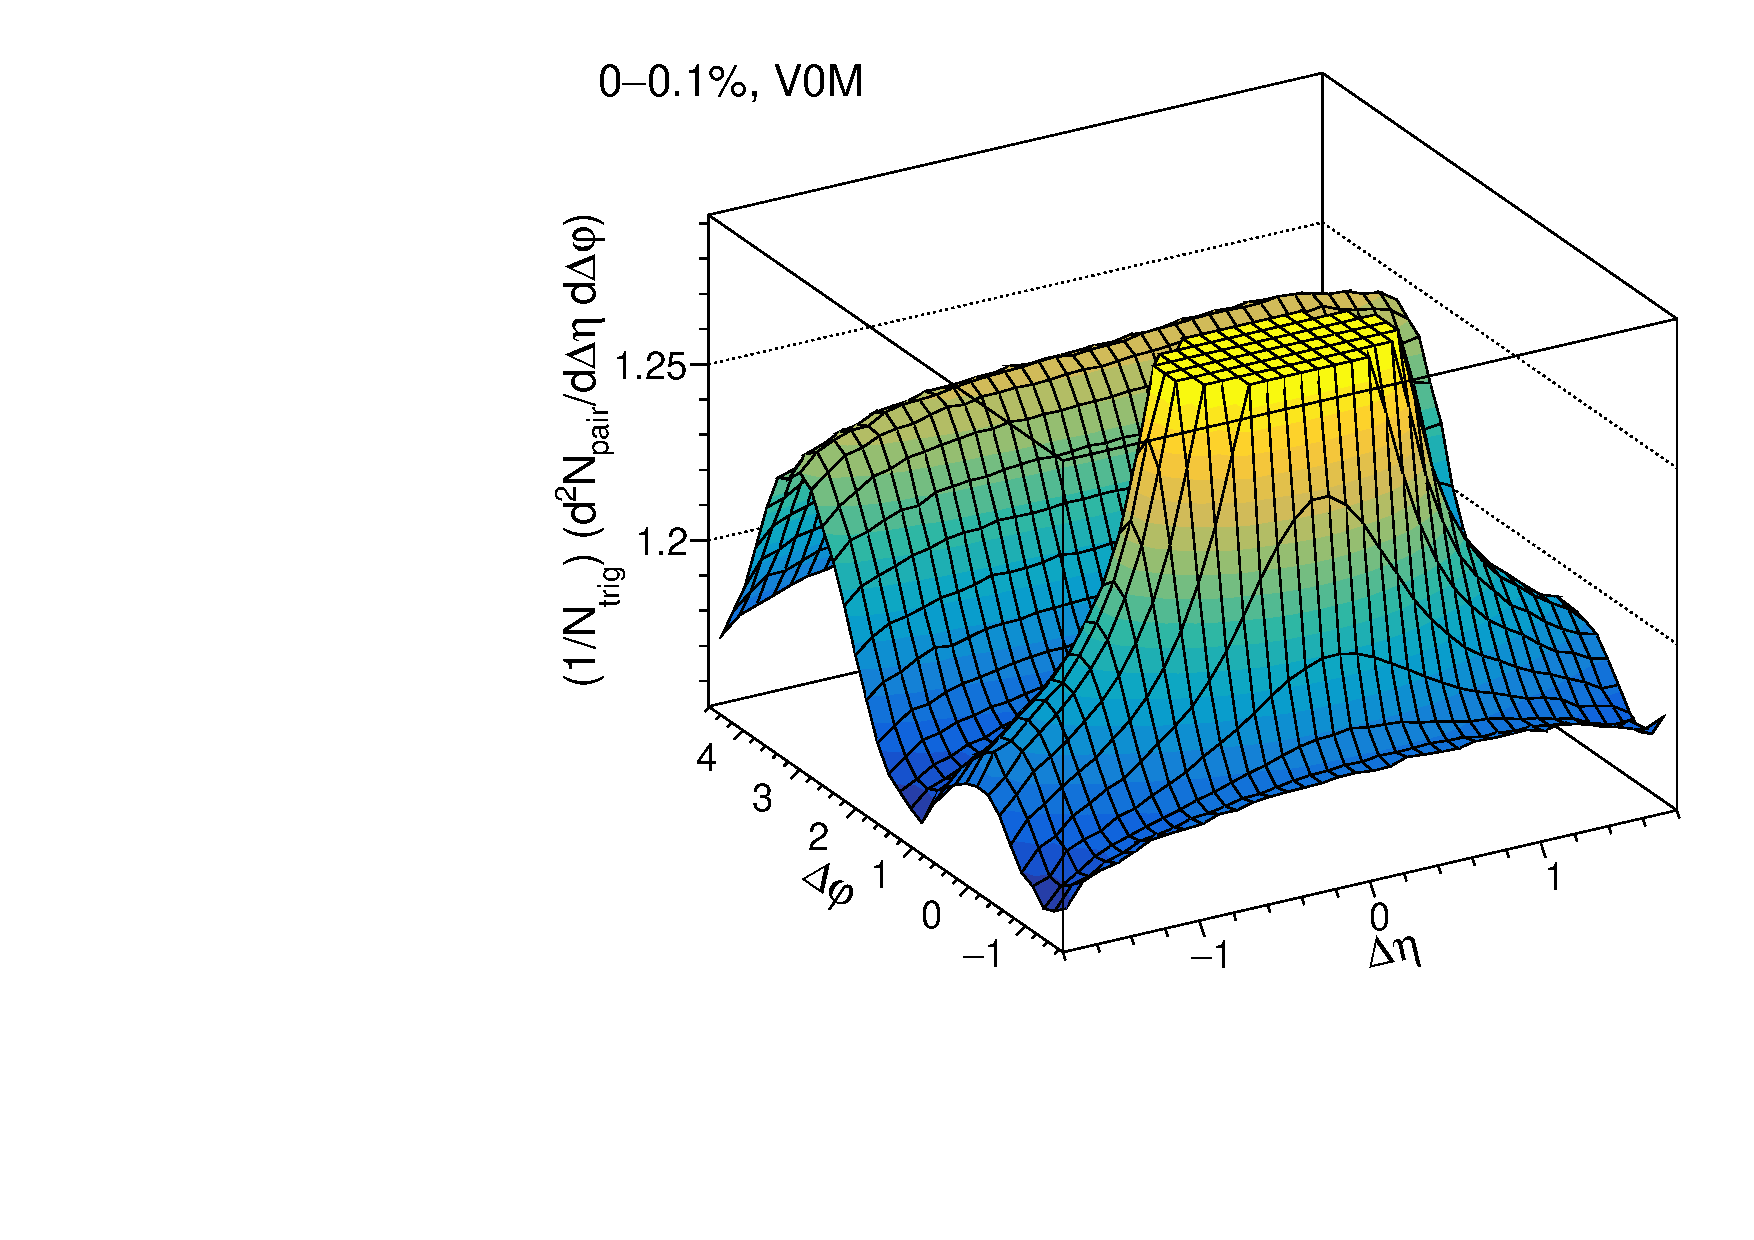
\includegraphics[width=0.5 \textwidth]{figures/Fig1_ppHigh.pdf} 
		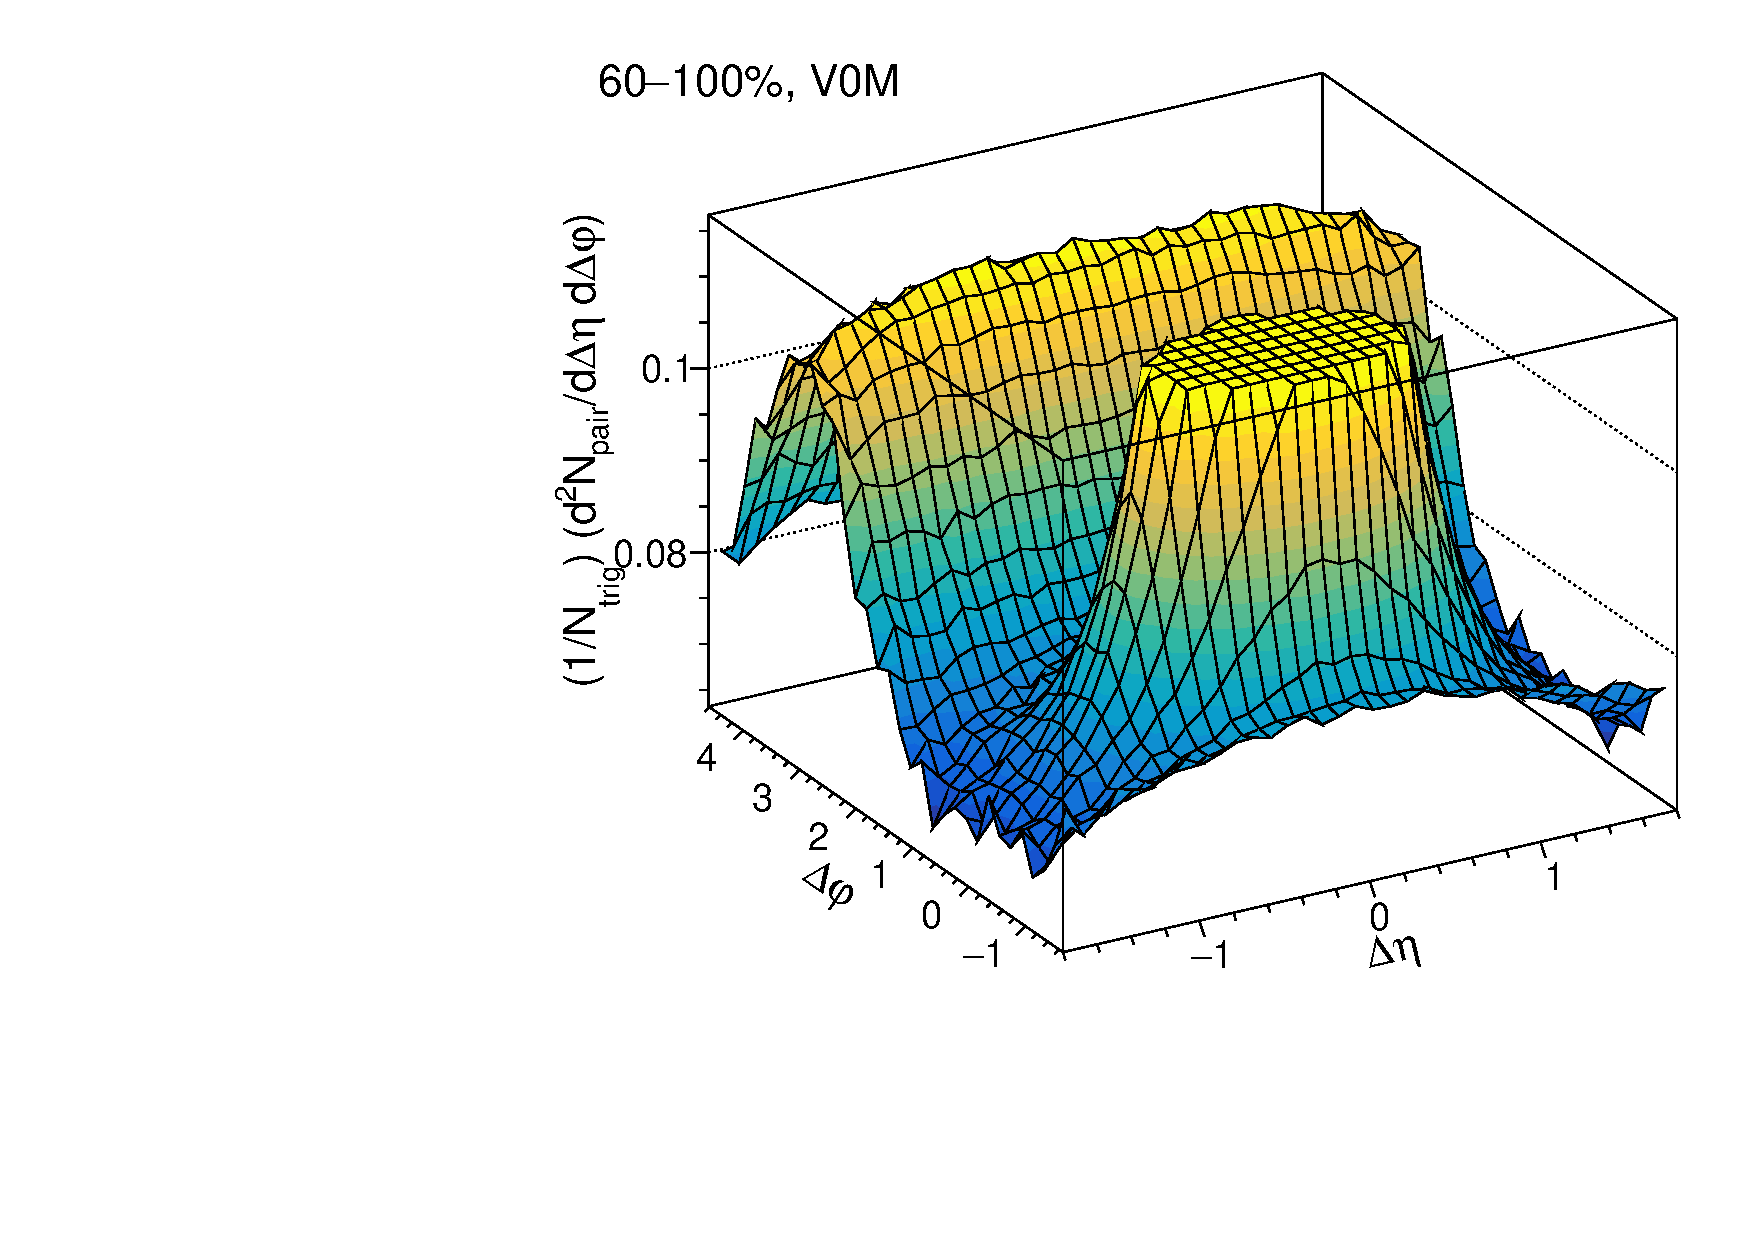
\includegraphics[width=0.5 \textwidth]{figures/Fig1_ppLow.pdf} 
  		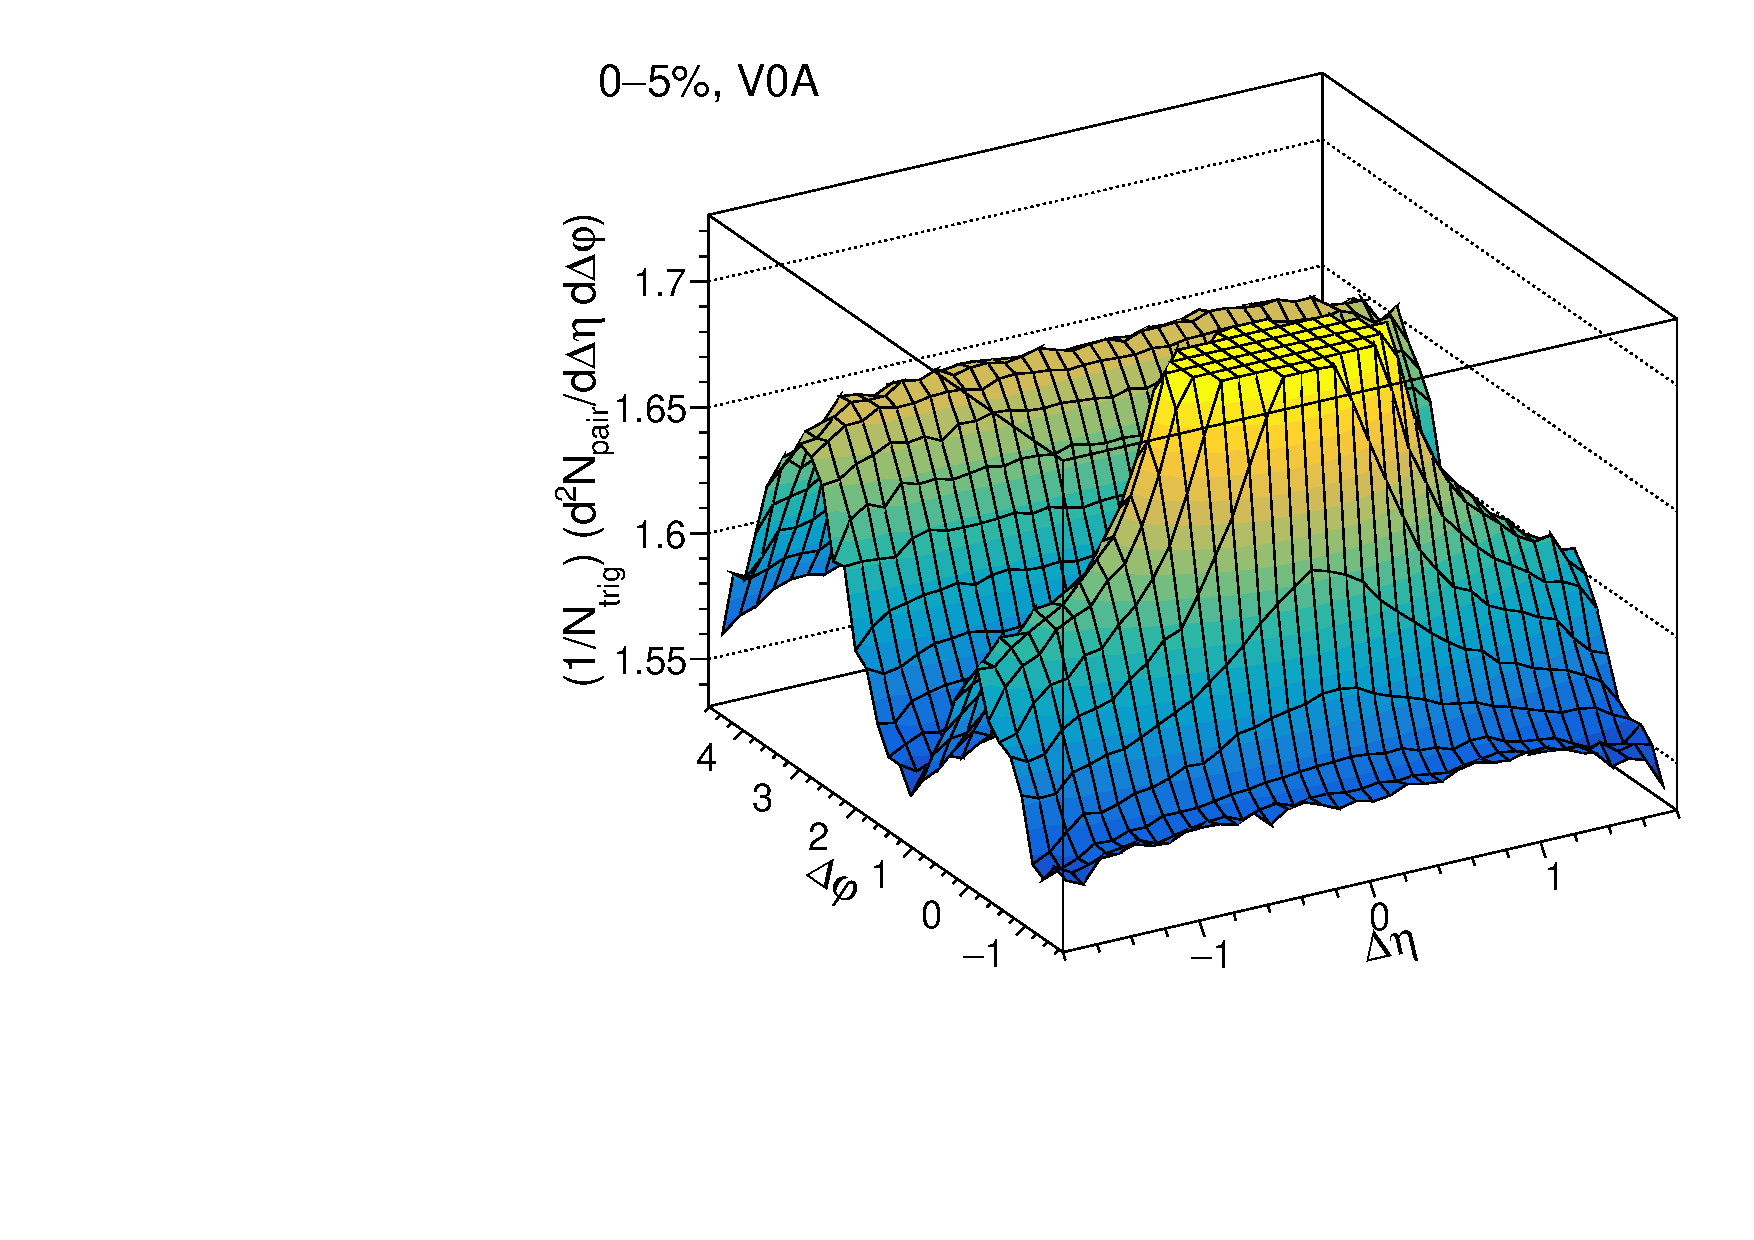
\includegraphics[width=0.5 \textwidth]{figures/Fig1_pPbHigh.pdf}
		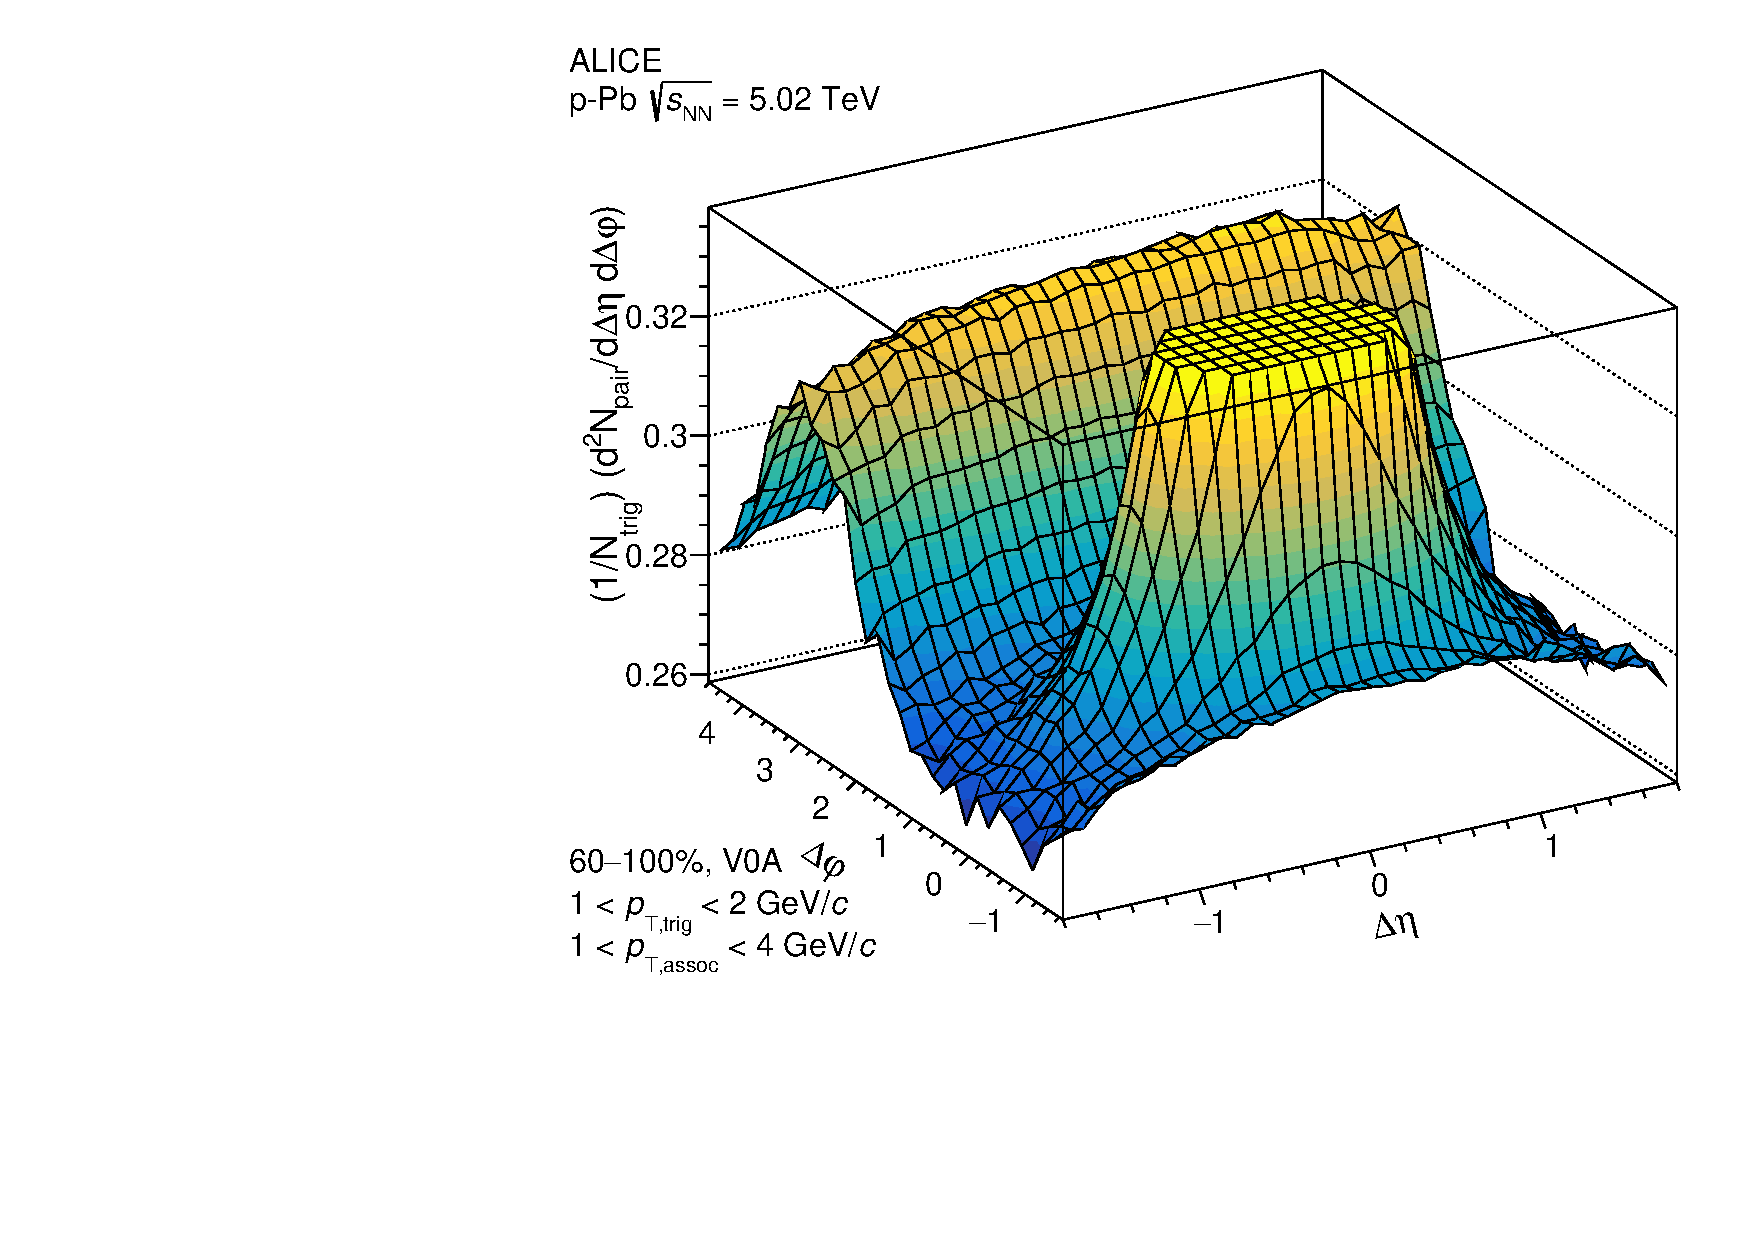
\includegraphics[width=0.5 \textwidth]{figures/Fig1_pPbLow.pdf}
\caption{The two-dimensional correlation functions as functions of $\Delta\eta$ and $\Delta\varphi$ are shown for HM (0--0.1\% or 0-5\%, on the left) and LM (60--100\%, on the right) events in $\sqrt{s}=13$ TeV pp collisions (top) and $\sqrt{s_{\mathrm{NN}}}=5.02$ TeV p--Pb collisions (bottom). The intervals of $\pttrig$ and $\ptassoc$ are 1~$<\it{p}_{\rm{T}}<$~2~GeV/$c$ in all cases.}
\label{fig:doubleridge}
\end{figure}

The two-dimensional correlation functions in pp collisions at $\sqrt{s}=13$ TeV are shown at the top panels in Fig.~\ref{fig:doubleridge} for the high-multiplicity (0--0.1\%, left) and low-multiplicity (60--90\%, right). The bottom panels show those in $\sqrt{s_{\mathrm{NN}}}=5.02$ TeV p--Pb collisions. The multiplicity percentile of p--Pb collisions is wider, ranging from 0--5\%, compared to that of pp collisions.
The $z$-axis for the correlation yield is properly scaled in order to zoom in the larger $\Delta\eta$ region. As a result, the jet peaks are sheared off in both figures. The flow modulation structure is clearly observed in the HM class for both systems while it is not seen in the LM-template. The away-side regions are populated mostly by back-to-back jet correlations but they are reduced and compatible to the one in near side in $\Delta\eta > 1.6$.

The per-trigger yield is extracted for various multiplicity percentiles and $\pt$ intervals at large $\Delta\eta$, at $1.6<|\Delta\eta|<1.8$ to remove the near-side non-flow contributions. The per-trigger yield as a function of $\Delta\varphi$ is expressed as
\begin{eqnarray}
Y(\Delta\varphi) = \frac{1}{N_{\rm{trig}}} \frac{ \rm{d}\it{}N_{\rm{pair}} }{ \rm{d}\Delta\varphi } = \int_{1.6<|\Delta \eta|<1.8} \left( \frac{1}{\it{N}_{\rm{trig}}} \frac{ \rm{d}\it{}^{2} N_{\rm{pair}} }{ \rm{d}\Delta\eta \rm{d}\Delta\varphi} \right) \dfrac{1}{\delta_{\Delta\eta}} \rm{d}\Delta \eta \quad ,
\label{eq:pertrigger}
\end{eqnarray}
where the factor $\delta_{\Delta\eta}=$~0.4 is used as a normalization to obtain the per trigger yield per unit of pseudorapidity.
%The Zero-Yield-At-Minimum (ZYAM) procedure~\cite{Ajitanand:2005jj} is the method used to subtract the baseline of the correlation. 


\subsection{Extraction of flow coefficients from the low-multiplicity template fit method}

As discussed in Refs.\cite{ATLAS:2015hzw,ATLAS:2016yzd}, the correlation function in a high multiplicity percentile is fitted with 
\begin{eqnarray}
\label{eq:narray}
Y_{\rm{HM}}(\Delta\varphi) = G~(1 + 2v_{2,2}\cos(2\Delta\varphi) + 2v_{3,3}\cos(3\Delta\varphi)) + F~Y_{\rm{LM}}(\Delta\varphi) \quad,
\end{eqnarray}
where $Y_{\rm{LM}}(\Delta\varphi)$ is the low-multiplicity template, G is the normalization factor for the Fourier component up to the third harmonic, and the scale factor $F$ corresponds to the relative away-side jet-like contribution with respect to the LM (the 60--100\%) template corresponding to the 60--100\% percentile. 
The fit determines the scale factor $F$, pedestal $G$, and $v_{n,n}$. This method does not rely on the zero yield at minimum (ZYAM) hypothesis~\cite{Ajitanand:2005jj} to subtract an assumed flat combinatorial component from the LM template as done previously in Refs.~\cite{ATLAS:2012cix,ATLAS:2014qaj}. 
This method assumes that $Y_{\rm{LM}}$ does not  contain a peak in the near side originating from jet fragmentation and that the jet shape remains unchanged in HM events compared to LM events.
The first assumption is well-verified using the selected LM template, while the second assumption regarding the modification of jet shapes is tested using the near-side $\Delta\eta$ distributions. Additionally, the ATLAS Collaboration's study of high-multiplicity pp and p-Pb collisions in Ref.~\cite{ATLAS:2018ngv} provides further support for this assumption, as there is no evidence of jet quenching in these collisions~\cite{Adam:2014qja,Khachatryan:2016odn,Adam:2016jfp,Adam:2016dau,Acharya:2017okq}.

\begin{figure}[h!]
	\centering
	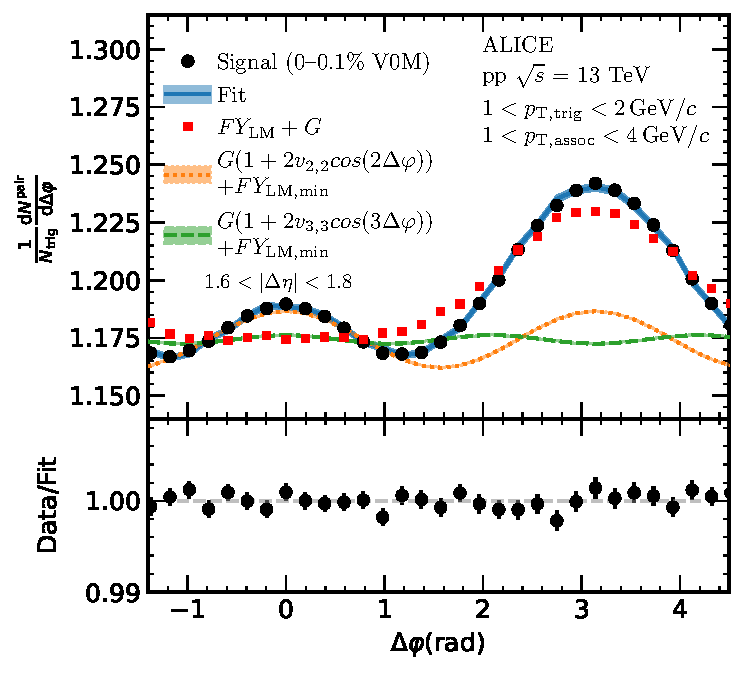
\includegraphics[width=0.6 \textwidth]{figures/Fig1_FlowExt.pdf} 
	\caption{The template fit results with the LM-templates. The black markers shows the signal for the $0-0.1\%$ multiplicity percentile together with its fit shown as a blue band. The red squares correspond to the LM signal. The orange and green curves correspond to the extracted $v_2$ and $v_3$ signals, respectively. The $\chi^{2}$ divided by the number of degree of freedom is 0.894}
	\label{fig:flowext}
\end{figure}

Figure~\ref{fig:flowext} shows the LM-template fit results for 0--0.1\% multiplicity percentile pp collisions at $\sqrt{s}$ = 13 TeV. The LM yield,  $Y_{\rm{LM}}(\Delta\varphi)$, is shown in red squares, and the extracted $v_{2}$ and $v_{3}$ as orange and green respectively. The results on the scale factor F in different multiplicity percentiles and systems are summarized in Tabs.~\ref{tab:Fpp} and \ref{tab:Fpb}. They are larger for pp higher multiplicity percentiles and closer to unity for p--Pb lower multiplicity percentiles. In the previous results in Refs.~\cite{ALICE:2012eyl,ALICE:2013snk} from 2012 and 2013, $F$ was assumed to be 1. The fit to the signal is shown as a blue band and the signal-to-fit ratio is shown in the bottom panel. 
%let's add chiq value of the fit
\begin{table}[h!]
\caption{The scale factor $F$ for various multiplicity percentiles in pp collisions.}
\centering
\begin{tabular}{|c|cccc|c}
\hline
 V0M& 0--0.1\% & 1--5\% & 5--20\% & 20--60\% \\ 
 \hline
 $F$ & 1.504$\pm$0.017 & 1.414$\pm$0.030 & 1.360$\pm$0.019 & 1.208$\pm$0.015 \\  
 \hline
 \end{tabular}
 \label{tab:Fpp}
 
\end{table}

\begin{table}[h!]
\caption{The scale factor $F$ for various multiplicity percentiles in p--Pb collisions.}
\centering
\begin{tabular}{|c|cccccc|c}
 \hline
 V0A& 0--5\% & 5--10\% & 10--20\% & 0--20\% & 20--40\% & 40--60\% \\ 
 \hline
 $F$& 1.135$\pm$0.026 & 1.140$\pm$0.026 & 1.152$\pm$0.021 & 1.145$\pm$0.017 &1.092$\pm$0.015 & 1.083$\pm$0.015 \\  
 \hline
\end{tabular}
\label{tab:Fpb}
\end{table}

\begin{figure}[h!]
	\centering
	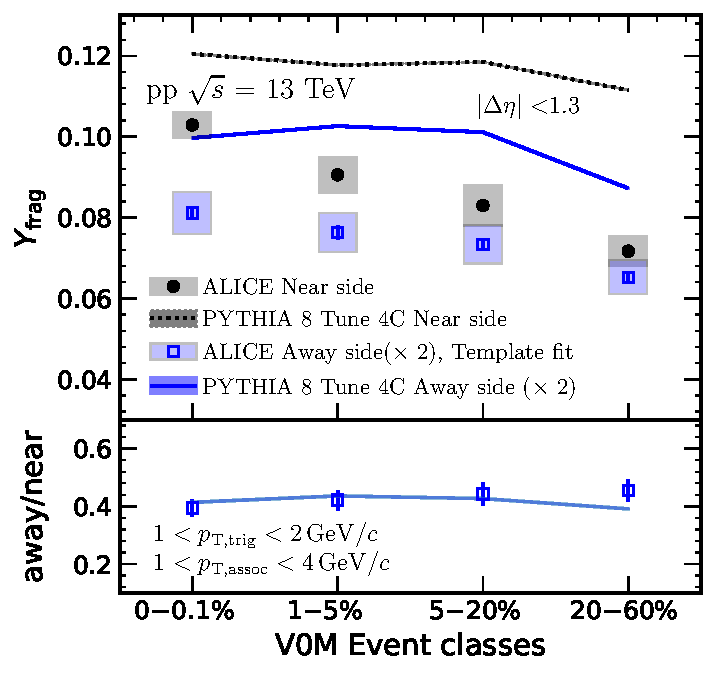
\includegraphics[width=0.6 \textwidth]{figures/Fig5_Plot_v2Mult.pdf} 
	\caption{The $Y^{\rm{frag}}$ for the near- and away-side as a function of multiplicity percentiles with both ALICE and PYTHIA data. The ratio includes the combined statistical and systematic errors in quadrature.}
	\label{fig:Ymult}
\end{figure}

The near-side jet-like yields are extracted from the near-side $\Delta\eta$ correlations, defined in $|\Delta\varphi|<$~1.3 as the following
\begin{eqnarray}
Y^{near}_{\rm{frag}} = \int_{|\Delta \eta|<1.3} \left( \frac{1}{\it{N}_{\rm{trig}}} \frac{ \rm{d}\it{}N_{\rm{pair}} }{ \rm{d}\Delta\eta } \right) \rm{d} \Delta\eta \quad.
\label{eq:Ynear}
\end{eqnarray}
%The range of $\Delta\varphi$ is chosen to be 1.3 in order for the projection range to fully cover the near-side peak in $\Delta\varphi$. 
The correlations in the same jet mainly contribute to $(\Delta\eta, \Delta\varphi) \sim (0,0)$ due to the similar out-going direction of particles inside the jet along the jet-axis. As can be seen in Eq.~\ref{eq:Ynear}, the yield of the jet fragmentation is calculated by integrating the $\Delta\eta$ correlation over $|\Delta\eta|<1.3$ after applying the ZYAM procedure~\cite{Ajitanand:2005jj}. The ZYAM procedure is applied by finding the minimum value of $\Delta\eta$ correlations within $|\Delta\eta|<1.3$, which results in pointing the minimum position to be $|\Delta\varphi|=1.3$.

The away-side jet-like yield in data is measured from the LM-template fit method as $Y^{\rm{away, HM}}_{\mathrm{frag}} = Y^{\rm{away, LM}}_{\mathrm{frag}} \times F$, where $F$ is the parameter from Eq.~\ref{eq:narray}. The $Y^{\rm{away, LM}}_{\mathrm{frag}}$ is then directly measured by integrating the away-side LM $\Delta\varphi$ correlation function. For the PYTHIA measurements, it is possible to directly measure $Y^{\rm{away}}$ from the $\Delta\varphi$ correlation functions since PYTHIA does not include any flow contributions.

Figure~\ref{fig:Ymult} presents the $Y^{\mathrm{near}}_{\rm{frag}}$ and $Y^{\mathrm{away}}_{\rm{frag}}$, for both ALICE data and PYTHIA 8 Tune 4C as a function of multiplicity percentile in pp collisions at $\sqrt{s}=13$ TeV. The transverse momentum range for trigger particles is $1<p_\mathrm{T,trig}<2$ GeV/c and for associated particles $1<p_\mathrm{T,assoc}<4$ GeV/c. ALICE data points are shown as circle and square markers, whereas PYTHIA is shown as lines. The near-side yields are shown in black and the away-side yields in blue.
The near- to away-side ratio for ALICE and PYTHIA data is shown in the bottom panel. While PYTHIA overestimates ALICE data for both $Y^{\mathrm{near}}_{\rm{frag}}$ and $Y^{\mathrm{away}}_{\rm{frag}}$, the ratio to PYTHIA is consistent with the ALICE data in the multiplicity percentiles studied. This ratio can be explained by the pair acceptance effect caused by the limited ALICE $\eta$ acceptance~\cite{PHENIX:2006gto}, which implies that the enhanced jet yields in away-side in HM events with respect to LM events are well quantified by the LM-template method.

%\begin{figure}[h!]
%		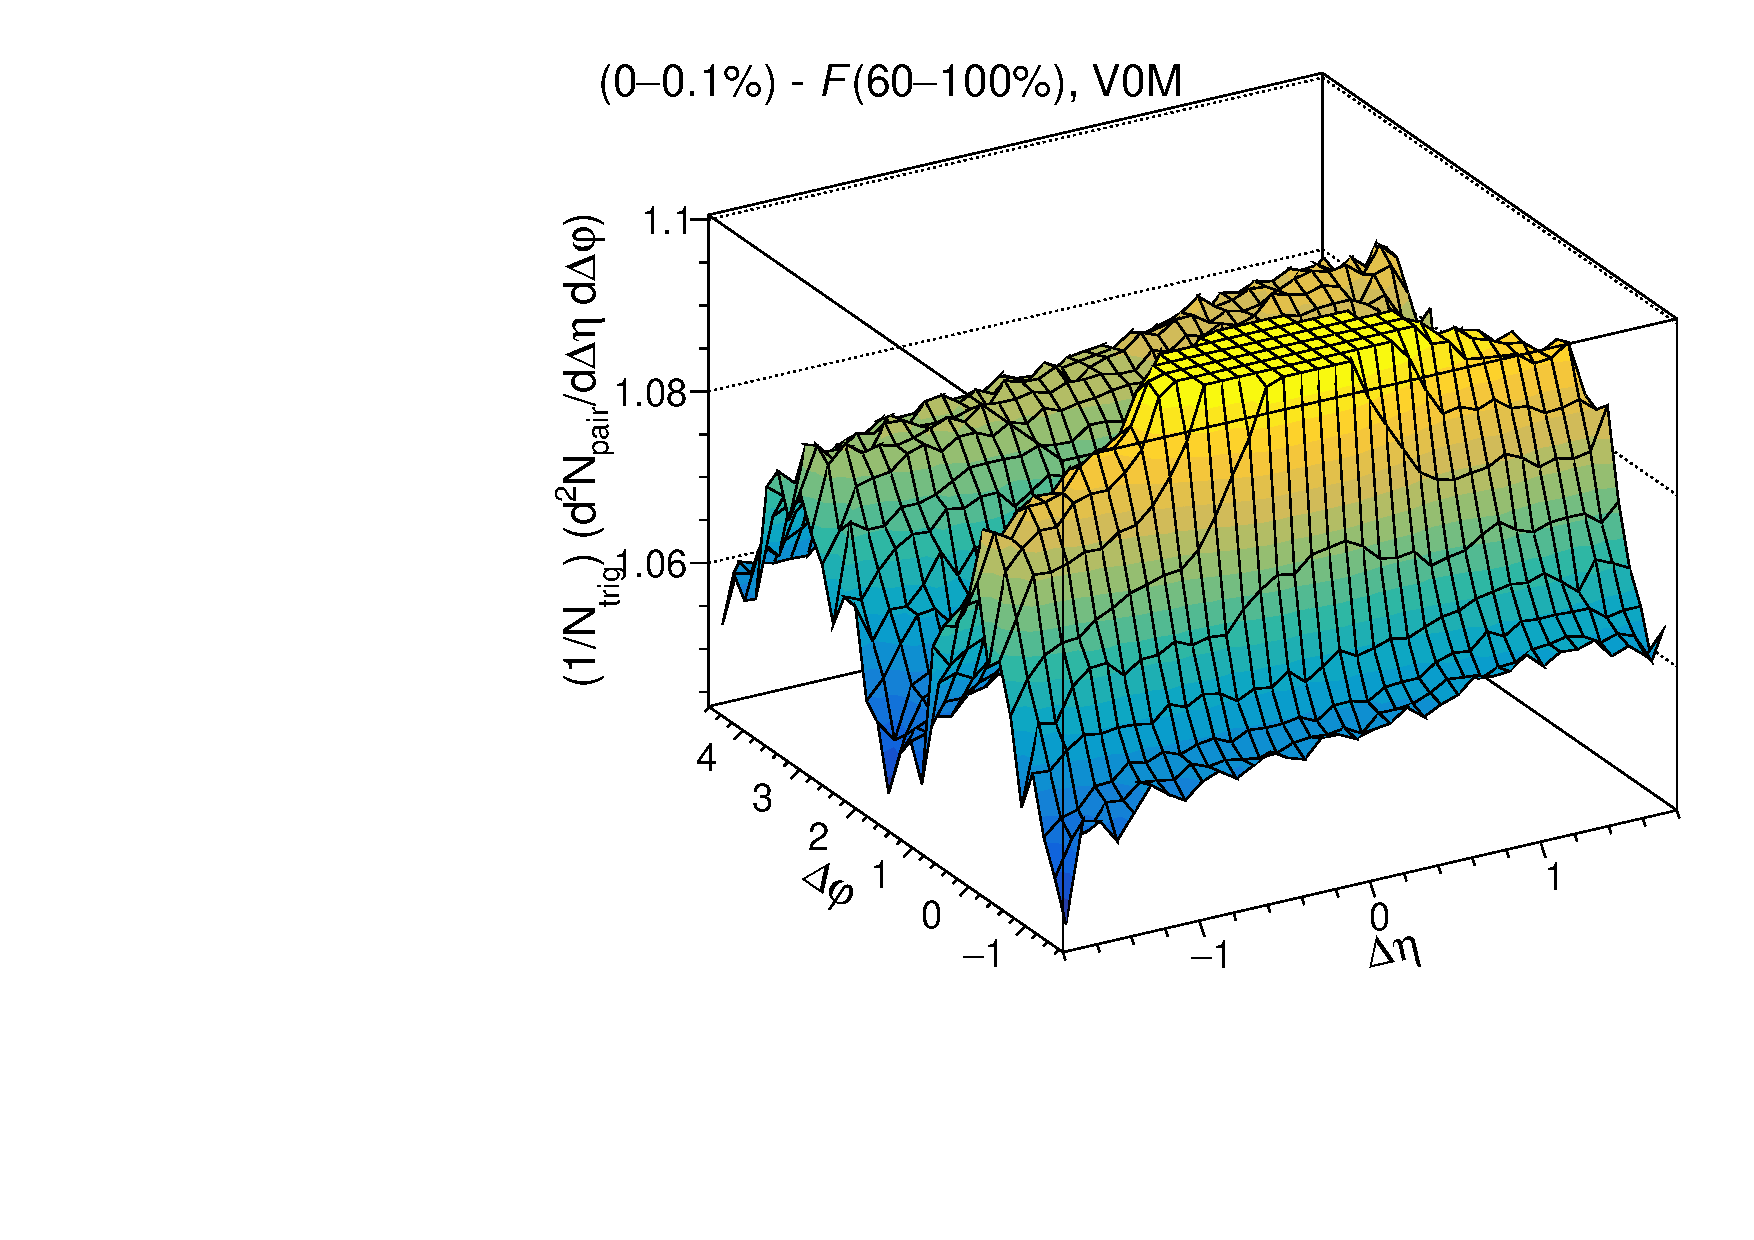
\includegraphics[width=0.5 \textwidth]{figures/Fig1_ppSub.pdf}
%  		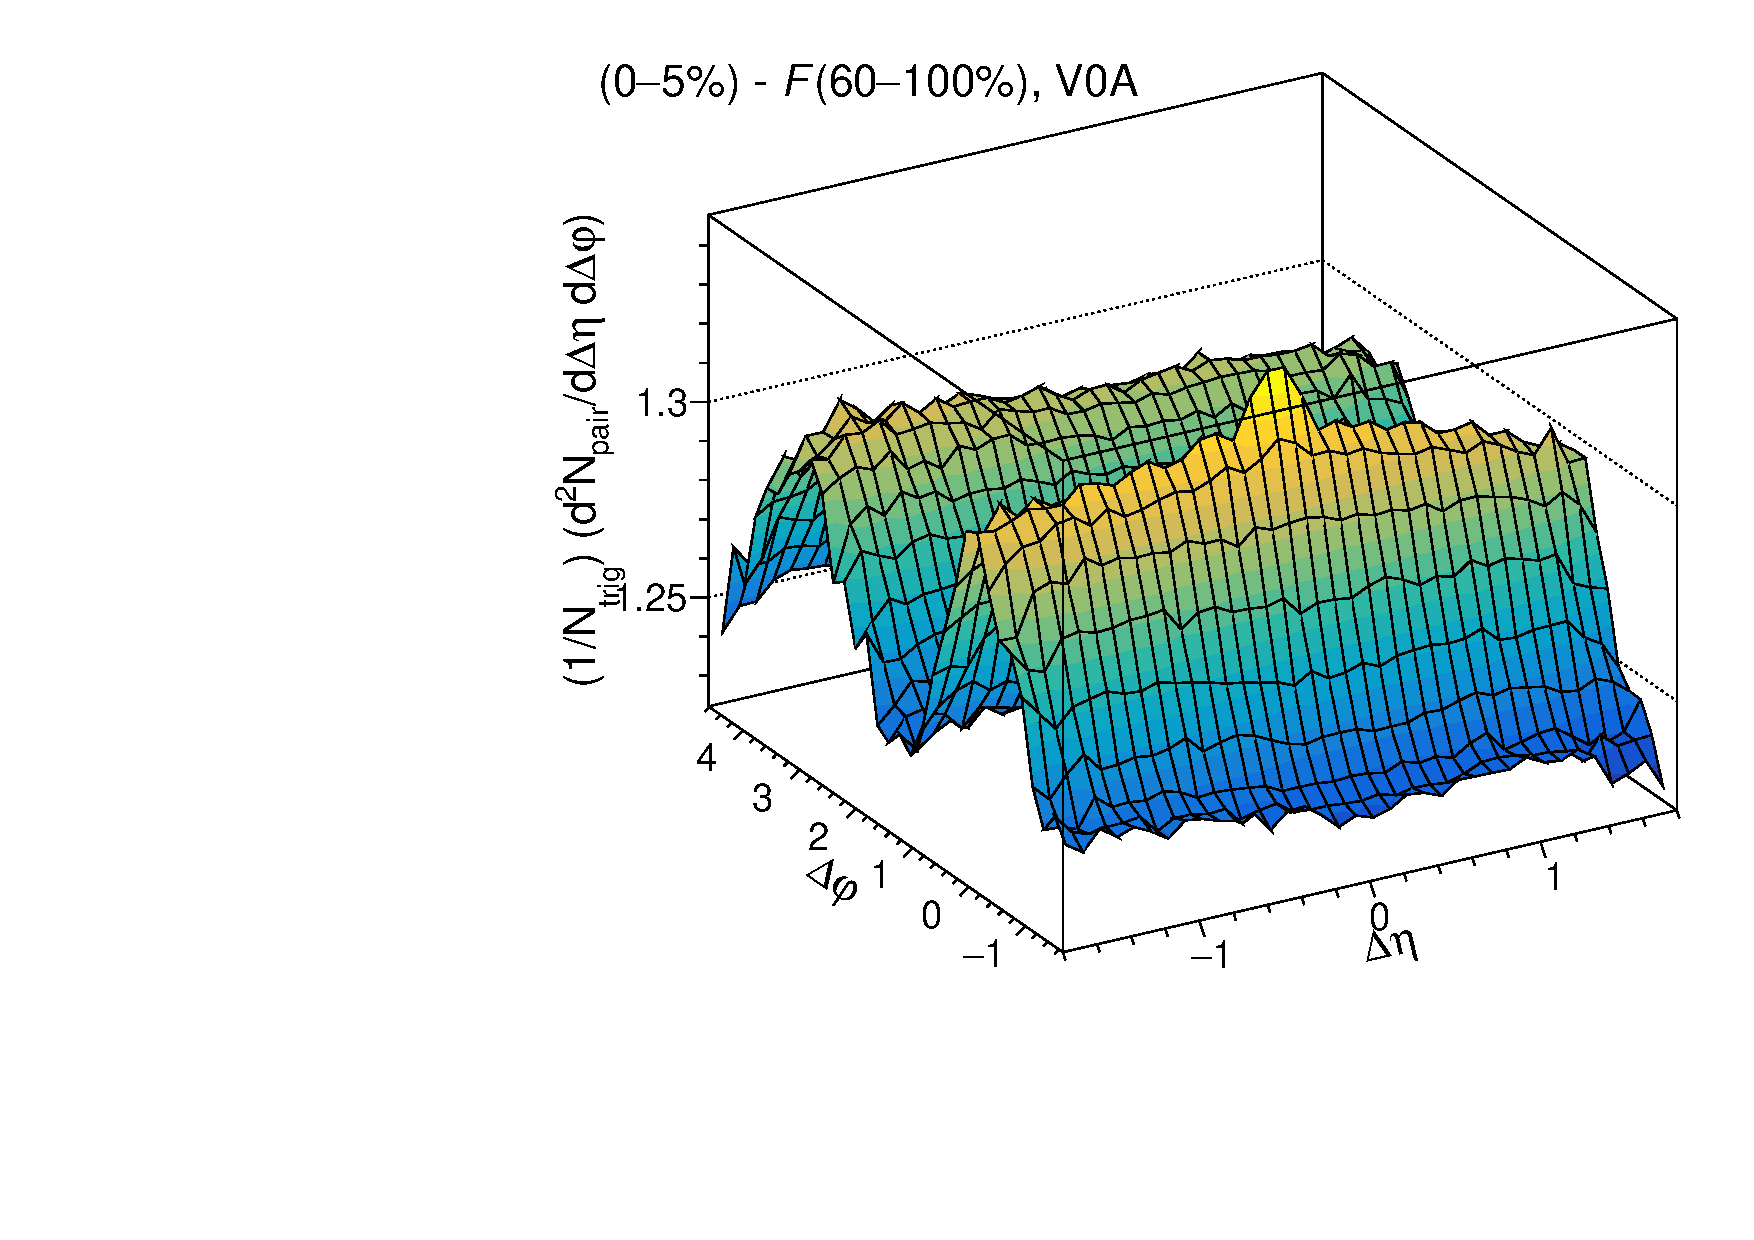
\includegraphics[width=0.5 \textwidth]{figures/Fig1_pPbSub.pdf}
%\caption{The subtracted one as (0--0.1)\%-$F$(60--100\%) is shown on the right. The subtracted one as (0--5)\%-$F$(60--100\%) is shown on the right. Note that the near-side jet peaks exceed the chosen range of the $z$-axis. The intervals of $\pttrig$ and $\ptassoc$ are 1~$<\it{p}_{\rm{T}}<$~2~GeV/$c$ in all cases.}
%\label{fig:doubleridge_sub}
%\end{figure}

%The subtracted one as (0--5)\%-$F$(60--100\%) on the right. Similarly, the ones in p--Pb collisions at $\sqrt{s_{\mathrm{NN}}}=5.02$ TeV are shown in Fig.~\ref{fig:doubleridge_sub}. The $F$ values can be found in Tables~\ref{tab:Fpp} and \ref{tab:Fpb}, which come from the LM-template fit in a given multiplicity percentile as described in Sec.~\ref{sec:ana}. 
%show an asymmetry in delta eta, e.g. in pp collisions the signal
%rises going from negative to positive delta eta values

The final step is to extract $v_{n}$, based on the observed factorization of $v_{n,n}$ to single harmonics~\cite{ATLAS:2015hzw,ATLAS:2016yzd}, using the following equation\quad,
\begin{eqnarray}
v_{n}(p_{\rm{T,trig}}) = v_{n,n}(p_{\rm{T,trig}}, p_{\rm{T,assoc}}) / \sqrt{ v_{n,n}(p_{\rm{T,assoc}},p_{\rm{T,assoc}})}
\end{eqnarray}
, where $v_{n,n}(p_{\rm{T,assoc}}$ and $p_{\rm{T,assoc}})$ are measured in 1~$<p_{\rm{T,trig}}<$~4~GeV/$c$ interval as the $p_{\rm{T,assoc}}$ range is fixed with 1~$<p_{\rm{T,assoc}}<$~4~GeV/$c$.
As a continuation of the extraction of the flow coefficients with the LM-template fit method, different event scale selections are investigated. By selecting events that includes a hard jet or a high-$\pt$ leading particle within the mid-rapidity region, it is possible to study the impact parameter dependence of flow coefficients in pp collisions~\cite{Sjostrand:1986ep,Frankfurt:2010ea}. This event scale is set by requiring a minimum $\pt$ of the leading track ($\ptlead$) or the reconstructed jet ($\ptjet$) at midrapidity. The leading particle track requires to be within $|\eta|<0.9$ and $0<\phi<2\pi$, and the jets are reconstructed with the anti-$k_{\rm{T}}$ algorithm~\cite{Cacciari:2008gp,Cacciari:2011ma}, with $R=0.4$ for only charged particles. In this analysis the $\pt$ scheme is used as the recombination scheme. In the same way as for the leading particle tracks, the jets are selected in the full azimuthal angle ($0<\phi<2\pi$) but in an $\eta$-range of $|\eta_\mathrm{jet}|<0.4$. The $\pt$ of jets $\ptjet$ is corrected for the underlying event density that is measured using the $k_{\rm{T}}$ algorithm with $R=$~0.2~\cite{Acharya:2018eat}.

%%%%%%%%%%%%%%%%%%%%%%%%%%%%%%%%%%%%%%%%%%%%%%%%%%%%%%%%%%

\section{Systematic uncertainties}
\label{sec:uncertainties}

\begin{table}[h!]
\caption{The relative systematic uncertainties of $Y^{\rm{near}}$, $Y^{\rm{away,LM}}$, $F$, $v_{2}$, and $v_{3}$. Numbers given in ranges correspond to minimum and maximum uncertainties. ``negl." is assigned if the systematic deviation is contaminated by the statistical fluctuation. ``N.A" is assigned when the systematic variation is not relevant to the measurement. }
\centering
\label{tab:syst}
\resizebox{\textwidth}{!} {
\begin{tabular}{c|ccccccc}
\hline 
\multirow{3}{*}{Sources}  & \multicolumn{7}{c}{Systematic uncertainty (\%)} \\ \cline{2-8} 
& \multirow{2}{*}{$Y^{\rm{near}}$} & \multirow{2}{*}{$Y^{\rm{away,LM}}$} & \multirow{2}{*}{$F$} & \multicolumn{2}{c}{$v_{2}$} & \multicolumn{2}{c}{$v_{3}$}  \\   \cline{5-8}
& & & & pp & p--Pb & pp & p--Pb  \\ \cline{1-8} 
Primary vertex       & $\pm$0.2--0.5 & $\pm$0.1      & $\pm$1.0--2.5 & $\pm$0.2--1.8 & $\pm$0.8 & $\pm$1.4 & $\pm$3.9 \\ 
Pileup rejection     & $\pm$0.1--0.5 & $\pm$0.2      & $\pm$0.4--1.5 & negl.         & $\pm$0.6 & negl. & $\pm$1.4 \\ 
Tracking		     & $\pm$1.0--3.0 & $\pm$2.0      & $\pm$0.6--2.4 & $\pm$0.2--3.0 & negl. & $\pm$5.0--6.9 & negl. \\ 
Event mixing	     & $\pm$0.2--0.7 & $\pm$0.2--0.5 & $\pm$0.0--3.3 & $\pm$0.3--4.6 & $\pm$0.8 & $\pm$2.8--3.1 & $\pm$0.8 \\ 
LM definition   	 & N.A.          & $\pm$0.5--3.5 & $\pm$0.7--6.0 & negl.         & $\pm$1.9 & negl. & $\pm$9.2\\ 
ITS-TPC matching 	 & $\pm$2.0--3.0 & $\pm$2.0--3.0 & N.A.          & N.A.          & N.A. & N.A. & N.A\\ 
Efficiency correction& $\pm$1.0--4.4 & $\pm$1.0--4.4 & N.A.          & N.A.          & N.A. & N.A. & N.A\\ 
$\eta$ gap range   	 & N.A.          & N.A.          & $\pm$0.1--3.2 & $\pm$1.0--5.0 & $\pm$0.4 & negl. & negl. \\ 

\hline 
Total (in quadrature)& $\pm$2.5--6.1 & $\pm$5.0--5.5 & $\pm$1.8--7.1 & $\pm$0.8--5.7 & $\pm$2.3 & $\pm$6.1--7.5 & $\pm$10.1 \\ 
\hline 
\end{tabular}
}
\end{table}

The systematic uncertainties of $Y^{\rm{near}}$, $Y^{\rm{away,LM}}$, and $F$ are estimated by varying the analysis selection criteria and corrections in pp collisions, while the systematic uncertainties of $v_{2}$ and $v_{3}$ are estimated in pp and p--Pb collisions. All systematic uncertainties are summarized in Table~\ref{tab:syst}.

The uncertainty associated to the selected range of the primary vertex is estimated by varying the accepted range from $|z_\mathrm{vtx}|<$~8~cm to $|z_\mathrm{vtx}|<$~6~cm. The variation of the range allows to test acceptance effects on the measurement. The estimated uncertainties of $Y^{\rm{near}}$ and $Y^{\rm{away,LM}}$ are 0.2--0.5\% and 0.1\%, respectively. The uncertainties associated with the primary vertex selection are estimated to be 1.0--2.5\%, 0.2--1.8\%, and 1.4--3.9\% for $F$, $v_{2}$, and $v_{3}$, respectively. 

Another source of systematic uncertainty is related to pileup rejection. Pileup events are rejected with the different rejection criteria such that the number of track contributors required for the reconstruction of pileup event vertices, where the number is changed from the default value of 3 to 5. The uncertainties of $Y^{\rm{near}}$ and $Y^{\rm{away,LM}}$ are estimated to be 0.1--0.5\% and 0.2\%, respectively. The estimated uncertainties are negligible for $F$. The estimated uncertainties of $v_{2}$ and $v_{3}$ are 0.6\% and 1.4\%, respectively.

The systematic uncertainty from the track selection criterion is estimated by employing another track selection criteria, denoted global tracks. Each global track is required to have at least one SPD hit. Due to inefficient parts of the SPD, the azimuthal distribution of global tracks is not uniform. The estimated uncertainty of observables for $v_{2}$ is 0.2--3.0\% and 5.0--6.9\% for $v_{3}$. 

An additional systematic uncertainty from the event-mixing is estimated by varying the interval of the primary vertex range, where events are mixed. The default value of 2~cm is changed to 1~cm. The resulting uncertainty of jet fragmentation yield ($Y^{\rm{near}}$ and $Y^{\rm{away,LM}}$) is 0.2--0.7\%. The uncertainties of $F$, $v_{2}$, and $v_{3}$ are estimated to be 0.3--4.6\%.

The systematic uncertainty from the LM definition is estimated by changing the range of the LM multiplicity percentile. There is no universal definition for the LM, and the default range for the LM in the present paper is set to 60--100\%, and changed to 70--100\%. The uncertainty of $Y^{\rm{away,LM}}$ is estimated to be 0.5--3.5\%. Note that the measurement of $Y^{\rm{near}}$ is not relevant to the LM definition, and the uncertainty is not estimated. The uncertainties of $F$, $v_{2}$, and $v_{3}$ are estimated to be 0.7--9.2\%.

The systematic uncertainty from matching the track reconstructed by the TPC and corresponding signal in the ITS is estimated by evaluating the fraction of the mismatch between them. The estimated uncertainties of $Y^{\rm{near}}$ and $Y^{\rm{away,LM}}$ are 2.0--3.0\%.

The systematic uncertainty from the efficiency correction for unidentified charged particles is estimated by evaluating the deviation between correlation functions that is constructed using true particles and correlation functions that is constructed using reconstructed tracks and corrected for the tracking efficiency. The estimated uncertainty is 0.1--5.0\%.

Due to the limited $\eta$-acceptance of the TPC, non-flow contributions mainly originating from jet fragmentations affect the flow measurement. As the shape of short range correlations mostly attributed to jet particles is getting broader with the decreasing $\pt$, the systematic uncertainty from $\eta$-acceptance is significantly dependent on the $p_{\rm{T}}$. To estimate the related uncertainty, the minimum $\Delta\eta$ gap is changed from 1.6 to 1.7 for constructing long-range $\Delta\varphi$ correlations.  The estimated uncertainties of $F$, $v_{2}$, and $v_{3}$ are 0.1--5.0\%.





 %ANNA
% !TEX root = paper.tex

\section {Results}
\label{sec:results}
\subsection{Transverse-momentum and multiplicity dependence of anisotropic flow}

\begin{figure}[!b]
	\centering
	\hspace{-3em}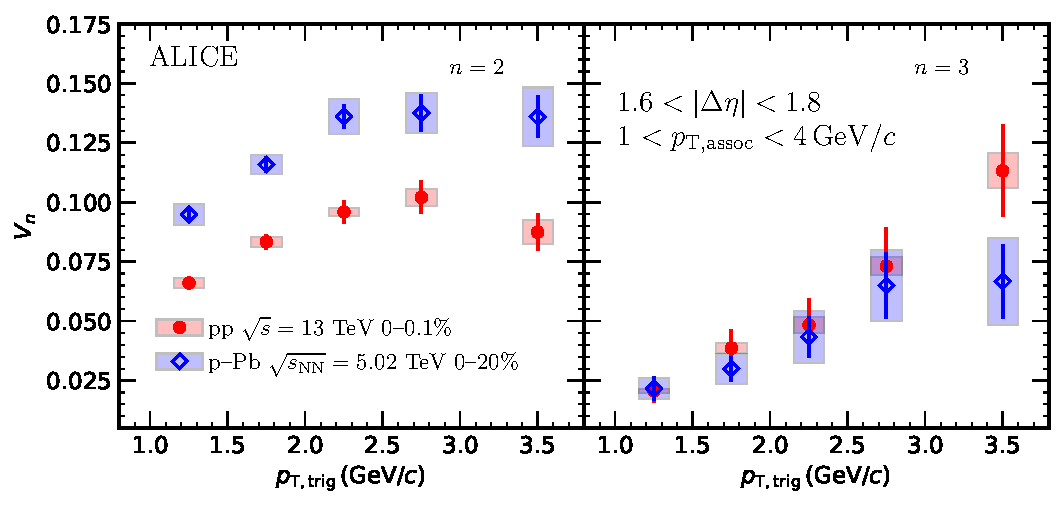
\includegraphics[width=0.9\textwidth]{figures/FIG4_vn_pppPb.pdf} %<--- keep the scale at 0.9 to match with other figures
	\caption{The magnitude of $v_2$ (left) and $v_3$ (right) as a function of $p_\mathrm{T}$ for the 0--0.1\% multiplicity interval in pp collisions at $\sqrt{s}=13$~TeV and 0--20\% in p--Pb collisions at $\sqrt{s_\mathrm{NN}} = 5.02$~TeV. The boxes around the data points represents the estimated systematic uncertainty and the error bars corresponds to the statistical errors.}
	\label{fig:vn}
\end{figure}
%python3 Fig2_vn_ppPb.py
Figure~\ref{fig:vn} illustrates the extracted values of $v_2$ and $v_3$ as a function of $p_{\mathrm{T,trig}}$ as obtained from Eq.~\eqref{eq:tmpfit}. The results correspond to the high-multiplicity pp collisions at $\sqrt{s}=13$~TeV and p--Pb collisions at $\sqrt{s_\mathrm{NN}}=$5.02~TeV. Both sets of results demonstrate an increasing trend in the magnitudes of $v_n$ with rising $p_{\mathrm{T,trig}}$. The $v_2$ data points reach a maximum between 2.5 and 3.0 GeV/$c$, similarly to what has been observed in Pb--Pb collisions~\cite{Abelev:2012di, ALICE:2018yph}.
The magnitudes of $v_2$ in p--Pb collisions are higher than those in pp collisions, which might be related to the larger p--Pb system size together with a likely longer lifetime of the hypothetically created medium.
However, the magnitudes of $v_3$ are similar in both systems, indicating that $v_3$ is less sensitive to the size of the systems.
These results are comparable to those obtained by ATLAS in different multiplicity classes, where the same method was used to extract the flow coefficients~\cite{ATLAS:2016yzd}. Even though the $\Delta\eta$ and $p_{\mathrm{T,assoc}}$ ranges used by ATLAS are wider, $2.0<|\Delta\eta|<5.0$ and $0.5<p_{\mathrm{T,assoc}}<5\,\mathrm{GeV}/c$, respectively, the results are consistent within uncertainties.

\begin{figure}[!t]
	\centering
%python3 Fig6_vn_allSystems_comp_dataonly.py
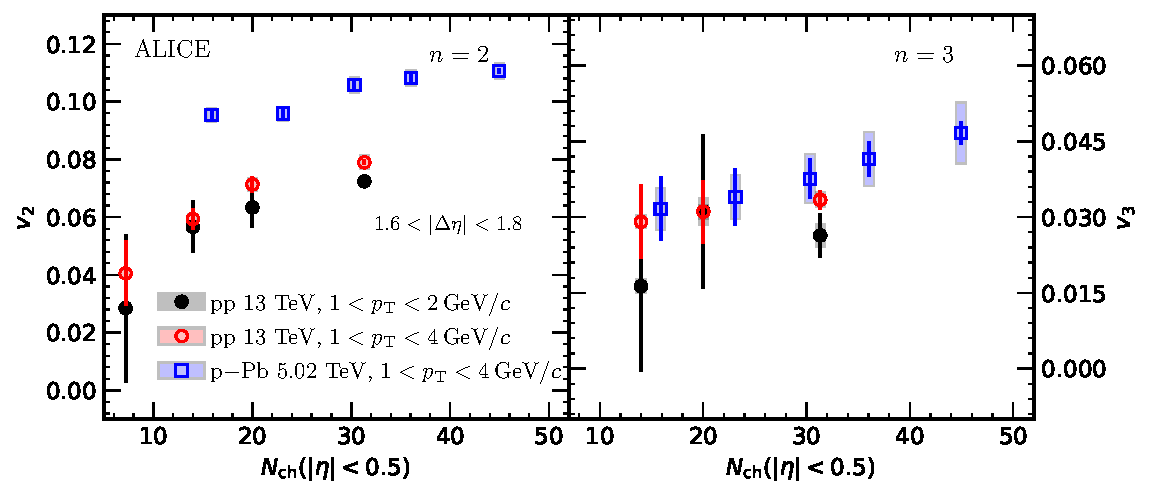
\includegraphics[width=1.0\textwidth]{figures/FIG5_v2Mult_allSystems_Data.pdf} 
	\caption{The magnitudes of $v_2$ (left
    panel) and $v_3$ (right panel) 
 for two different collision systems, pp and p--Pb as a function of charged-particle multiplicity at midrapidity. For pp collisions, two different $p_\mathrm{T}$-intervals are shown, $1.0<p_\mathrm{T}<2.0$ GeV/$c$ and $1.0<p_\mathrm{T}<4.0$ GeV/$c$. The boxes around the data points represent the estimated systematic uncertainties and the error bars corresponds to the statistical errors.} 
	\label{fig:v2mult}
\end{figure}

Figure~\ref{fig:v2mult} presents the magnitudes of $v_2$ and $v_3$, as a function of charged-particle multiplicity in the midrapidity for both pp collisions at $\sqrt{s}=13$ TeV and p--Pb collisions at $\sqrt{s_\mathrm{NN}}=5.02$ TeV. As in Fig.~\ref{fig:vn}, the $\Delta\eta$ gap is $1.6<|\Delta\eta|<1.8$ and $v_2$ is measured in $1<p_{\mathrm{T}}<4\,\mathrm{GeV}/c$ for both collision systems. Additionally, the corresponding results for pp collisions at $\sqrt{s}=13$ TeV with $1<p_{\mathrm{T}}<2$ GeV/$c$ are presented. First, it is observed that the magnitude of $v_n$ increases with increasing multiplicity for both collision systems and $p_\mathrm{T}$-ranges. Second, $v_2$ in p--Pb is higher than in pp collisions in the measured multiplicity range. These two observations are compatible with previous results from Refs.~\cite{ATLAS:2015hzw,ATLAS:2016yzd, Khachatryan:2015lva}. There is no significant difference between the two collision systems when considering the $v_3$ dependence on multiplicity as shown on the Right-hand-side panel of Fig.~\ref{fig:v2mult}. The $v_3$ measurements exhibit a comparable, subtle dependence on multiplicity, with higher values observed in collisions with greater particle multiplicities.
For the two different $p_\mathrm{T}$ intervals presented for the pp collisions, the $v_2$ in $1.0<p_\mathrm{T}<4.0$ GeV/$c$ shows a hint of larger magnitude than the $v_2$ in $1.0<p_\mathrm{T}<$~2.0~GeV/$c$. The difference in magnitude is significant only in the highest multiplicity point. 
This agrees with what is observed in Fig.~\ref{fig:vn}, where the $v_2$ magnitude has its largest value in $2.5<p_\mathrm{T}<$~3.0~GeV/$c$. It is found that for the considered $p_\mathrm{T}$ selections, the observed multiplicity dependencies differ only marginally. 
It is worth noting that the results presented from pp and p--Pb collisions were obtained from two different beam energies. In Ref.~\cite{ATLAS:2016yzd}, it was found that the magnitudes of $v_2$ and $v_3$ in pp collisions between 13 and 5.02 TeV show no significant variation with center-of-mass energy.

\subsection{Event-scale dependence of the flow coefficients}
\begin{figure}[h!]
	\centering
	\hspace{-3em}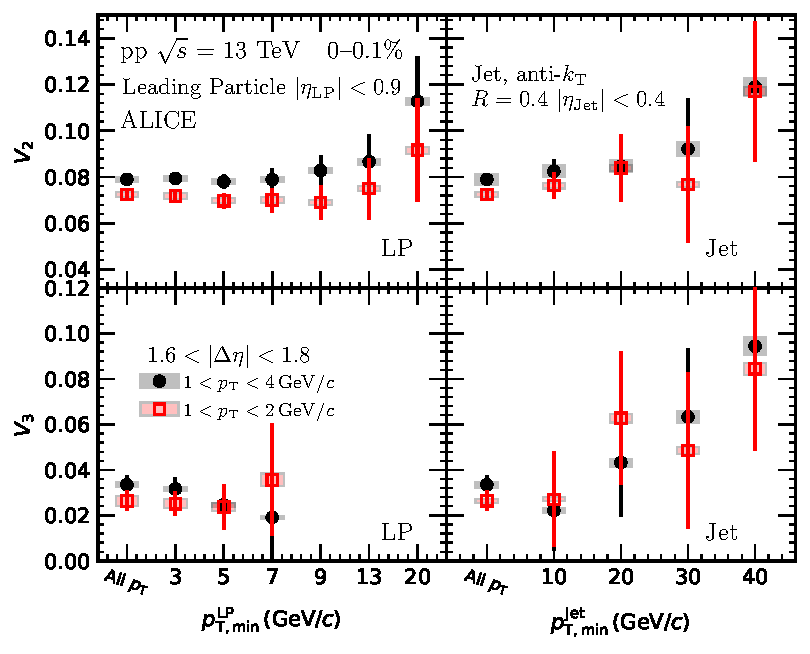
\includegraphics[width=0.8\textwidth]{figures/FIG6_vn_LP.pdf}
	\caption{The magnitudes of $v_2$ (top) and $v_3$ (bottom) as a function of $\it{p}^{\rm{LP}}_{\rm{T,min}}$ (left) and $\it{p}^{\rm{Jet}}_{\rm{T,min}}$ (right) for the high-multiplicity in pp collisions at $\sqrt{s}=13$. The measured $p_{\mathrm{T}}$ intervals are $1<p_{\mathrm{T}}<2\,\mathrm{GeV}/c$ (in red) and $1<p_{\mathrm{T}}<4\,\mathrm{GeV}/c$ (in black). The statistical errors and systematic uncertainties are shown as vertical bars and boxes, respectively.}
	\label{fig:LPjet23}
\end{figure}    

Figure~\ref{fig:LPjet23} presents the extracted magnitude of $v_2$ and $v_3$ as a function of the minimum $p_\mathrm{T}$ of the leading particle $\it{p}^{\rm{LP}}_{\rm{T,min}}$ and that of the jet ($\it{p}^{\rm{jet}}_{\rm{T,min}}$) as introduced in Sec.~\ref{sec:intro}. 
The results are presented for the 0–0.1\% multiplicity class of pp collisions at $\sqrt{s}= 13$ TeV and for the two different pT-ranges.
To reduce the impact of the detector edge effects on the jet measurements, the jet axes are required to have a pseudorapidity $|\eta_\mathrm{jet}|<0.4$, following a similar selection as in Refs.~\cite{CDF:2001onq, ATLAS:2014riz, CMS:2015jdl}. The $v_2$ and $v_3$ values for both $p_\mathrm{T}$ ranges do not show any dependence on event-scale selection within the uncertainties. This finding is consistent with the results of the ridge yields~\cite{ALICE:2021nir} and $v_{2}$ measurements with a tagged $Z$ boson from the ATLAS collaboration~\cite{Aaboud:2019mcw}. These results suggest that the presence of a hard-scattering process does not significantly change the long-range correlation involving soft particles.
However, the presented measurements are only limited to the low $\it{p}^{\rm{jet}}_{\rm{T}}$. Future measurements with multi-jet events at midrapidity with higher $Q^2$ reach can shed more light on the expected impact parameter dependence~\cite{Sjostrand:1986ep,Frankfurt:2003td,Frankfurt:2010ea}.

\subsection{Comparisons with models}
\label{sec:theory}

\begin{figure}[h!]
	\centering
	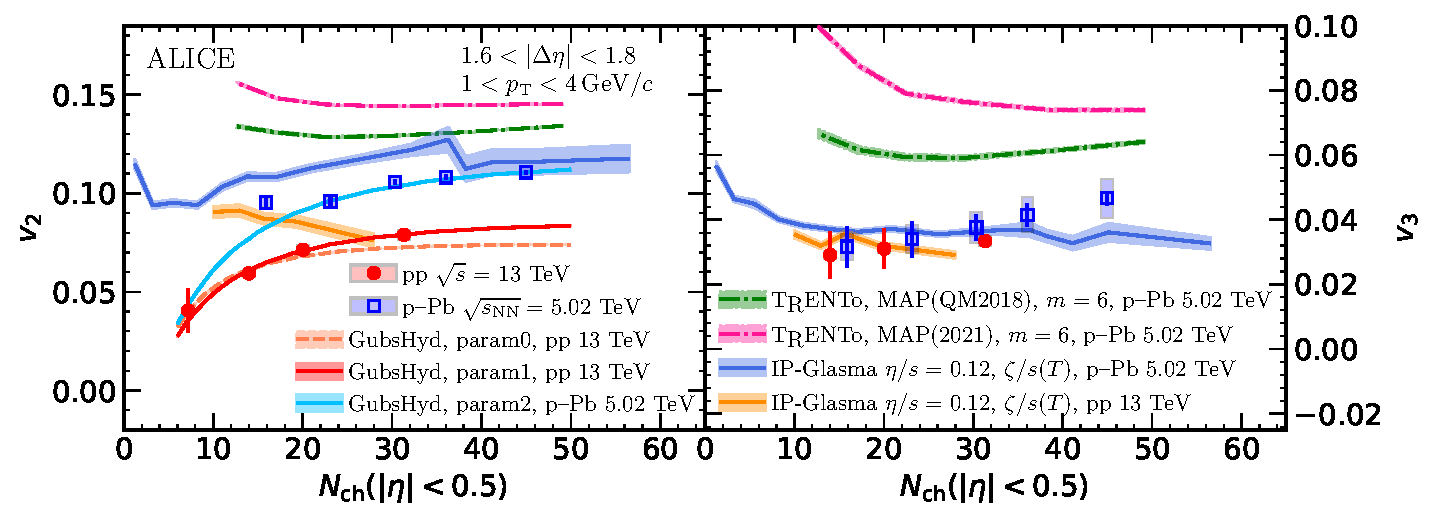
\includegraphics[width=1.0\textwidth]{figures/FIG7_v2Mult_allSystems_Hydro.pdf} 
	\caption{The measured and calculated evolution of $v_2$ (left) and $v_3$ (right) in pp and p--Pb collisions as a function of charged-particle multiplicity at midrapidity.
The blue and red markers represent the measured p--Pb and pp data, respectively. The calculations are provided by hydrodynamical models~\cite{Parkkila:2021yha,Bernhard:2016tnd,Schenke:2020mbo,Taghavi:2019mqz} are presented with colored lines. The corresponding bands mark their statistical uncertainty. For GubsHyd calculations, the statistical uncertainty is smaller than the line thickness.} 
	\label{fig:vnmult_model}
\end{figure}

In this section, the results are compared to various model calculations.
The results from p--Pb collisions are compared with hydrodynamic calculations using the parameterization from an improved global
Bayesian analysis. The analysis involves new sophisticated collective flow observables as obtained from two different beam energies in Pb--Pb collisions~\cite{Parkkila:2021yha}, constraining the initial conditions and transport properties of the QGP. This hydrodynamic model, {T\raisebox{-.5ex}{R}ENTo}+iEBE-VISHNU, consists of the {T\raisebox{-.5ex}{R}ENTo} model~\cite{Moreland:2014oya} to simulate the initial condition, which is connected with a free streaming to a 2+1 dimensional causal hydrodynamic model VISH2+1~\cite{Shen:2014vra}. The evolution is continued after hadronization with a hadronic cascade model (UrQMD)~\cite{Bass:1998ca,Bleicher:1999xi}.
 %The initial conditions, the shear viscosity to entropy density ratio $\eta/s(T)$, the bulk viscosity $\zeta/s(T)$, and other free parameters of the hybrid model are extracted in a global Bayesian analysis.
A model calculation is performed using the best-fit parameterization for transport coefficients selected based on maximum a posteriori (MAP) for Pb--Pb collisions at $\sqrt{s_{\text{NN}}}=5.02$~TeV. Two different MAP values are used for the calculations. They are based on Ref.~\cite{Parkkila:2021yha} and Ref.~\cite{Bernhard:2016tnd} and in Fig. 7 they
are labeled MAP(2021) and MAP(QM2018), respectively.
 The parameterization for the initial conditions, which include a sub-nucleon structure with six constituent partons per nucleon ($m=6$), is taken from a model calibration with additional p--Pb data~\cite{Moreland:2018gsh}. All kinematic selections, such as the transverse momentum and pseudorapidity intervals, are matched to the data reported in this article. The flow coefficients in the hydrodynamic calculation are extracted with the two-particle cumulant method, as the {T\raisebox{-.5ex}{R}ENTo}+iEBE-VISHNU does not contain any non-flow.

Figure~\ref{fig:vnmult_model} shows that {T\raisebox{-.5ex}{R}ENTo}+iEBE-VISHNU overestimates both $v_2$ and $v_3$. In the studied range, the $v_2$ and $v_3$ data increase with multiplicity. However, {T\raisebox{-.5ex}{R}ENTo}+iEBE-VISHNU predicts the opposite trend, which is similar to what is found in large collision systems~\cite{Acharya:2020taj}. The large discrepancies in the prediction might be alleviated by inclusion of the newly measured p--Pb constraints in a future Bayesian parameter estimation as well as by improvements of the initial condition model for small-system collisions.

The results are also compared with IP-Glasma+MUSIC+UrQMD hydrodynamic calculations~\cite{Schenke:2020mbo}. This model uses IP-Glasma initial conditions~\cite{Schenke:2012wb} including sub-nucleonic fluctuations with three hot spots per nucleon. The hydrodynamic evolution is performed by MUSIC~\cite{Schenke:2010rr} and coupled with UrQMD~\cite{Bass:1998ca,Bleicher:1999xi}, which performs hadronic cascade. 
The model calculations are performed assuming constant $\eta/s=0.12$ and a temperature dependent $\zeta/s(T)$~\cite{Rose:2020lfc}. 
This model describes well the multiplicity dependence of $v_2$ in p--Pb collisions and the magnitude at the highest multiplicity within the statistical uncertainties of the model but overestimates the data for the lower multiplicity classes. As for pp collisions, the calculations clearly miss both the observed magnitude except for $N_\mathrm{ch}>25$ as well as the trend of the multiplicity dependence. The model shows that $v_2$ decreases with increasing multiplicity, while the experimental result shows the opposite.
For $v_3$, the model accurately describes the magnitudes and multiplicity dependence across the measured multiplicity ranges. The magnitudes of $v_3$ are slightly smaller in pp collisions than in p--Pb collisions according to the calculations, which agrees with the data within the uncertainties. The level of agreement between data and the IP Glasma model calculations is found to be similar to the results reported in Ref.~\cite{Acharya:2019vdf}.

Finally, the results are compared with the GubsHyd model, a semi-analytical model based on the analytical Gubser solution to hydrodynamic equations~\cite{Gubser:2010ze,Gubser:2010ui}, known as Gubser flow. In Gubser flow, the initial state of conformal matter is linearly perturbed by an initial elliptic shape. The model is employed to shed light on the possible sources of the observed discrepancy between more realistic models mentioned above and the measurements in pp collisions~\cite{Taghavi:2019mqz}. Instead of modeling the initial entropy density in this model, as it is typically done in T$_{\text{R}}$ENTo or IP-Glasma, the initial state fluctuation is modeled directly. It assumes that proton ellipticity $\epsilon_{2}$ and RMS radius $r_{\text{rms}}$ fluctuate independently. These fluctuations are described by Gaussian probability distributions, which have widths $\sigma_{\epsilon}$
 and $\sigma_{r}$, respectively. The multiplicity dependence of two-particle correlation functions' $v_2\{2\}$ depends on $\sigma_{r}$ and  $\chi\sigma_{\epsilon}$, where the coefficient $\chi$ encapsulates a correction for idealizations used in GubsHyd, including the absence of dissipation effects. The values of $\sigma_{r}$ and  $\chi\sigma_{\epsilon}$, were obtained by comparing the model with data. Since no non-flow effect is considered in the calculation, $v_2\{2\}$ is comparable with the flow measurements in the present study. The calculations for two sets of parameters are compared
to data in Fig.~\ref{fig:vnmult_model}. The “param0” parameterization is based on the prediction proposed in Ref.~\cite{Taghavi:2019mqz} that $\chi \sigma_{\epsilon} =$ 0.097 and $\sigma_{r} =$ 0.4 fm. The other parameterizations “param1” and “param2” employ different $\chi \sigma_{\epsilon}$  and $\sigma_{r}$ values. The model captures the multiplicity dependence of $v_2$ well.

In summary, the measured value of $v_{2}$ decreases with decreasing multiplicity in both pp and p--Pb collisions. This trend is also predicted by GubsHyd model calculations (Refs.~\cite{Taghavi:2019mqz} and~\cite{Weller:2017tsr}). Interestingly, the opposite trend is observed for the IP-GLASMA+MUSIC+UrQMD hydrodynamic calculations of $v_2$, where the value decreases with increasing charged-particle multiplicity~\cite{Schenke:2020mbo}.
Approaching a lower bound for the size of a hydrodynamized
system as predicted in Ref.~\cite{Taghavi:2019mqz}, 
the decreasing trend of $v_2$, obtained by lowering the charged-particle multiplicity, changes and turns out to raise again after the observed minimum. However, this change in multiplicity dependence of $v_2$ at low multiplicities is still challenging to test with the current experimental uncertainties. For $v_3$, the IP-Glasma+MUSIC+UrQMD hydrodynamic calculations~\cite{Schenke:2020mbo} are the only ones that accurately describe its magnitude and multiplicity dependence across the measured ranges. The calculations predict that the magnitudes of $v_3$ are slightly smaller in pp collisions than in p--Pb collisions, within the measured multiplicity ranges. The discrepancies between the predictions and the data can be further studied by including these measurements in a future Bayesian parameter estimation, as well as by improving the initial-condition model for the small-system collisions.
 %JASPER
% !TEX root = paper.tex

\section{Conclusions}
\label{sec:summary}
Long-range correlations for pairs of charged particles with two-particle angular correlations are studied in ${\sqrt{{\textit s}}}=13$~TeV pp and ${\sqrt{{\textit s_{NN}}}}=5$~TeV p--Pb collisions. Fourier coefficients extracted from the long-range correlations ($\Delta\eta > 1.6$) in various high-multiplicity classes are extracted from the low-multiplicity template fit method which allows one to subtract the enhanced away-side jet yields in high-multiplicity with respect to low-multiplicity events. These results show a weak multiplicity dependence on $v_2$ both for pp and p--Pb collisions, a hint of disappearing $v_2$ signal below $N_{ch}$=10 in $\eta|<0.5$. Furthermore, the events with hard probes such as jets or leading particles doesn't show any changes in $v_2$ within the uncertainties. %ALL

%%%%% acknowledgements
\newenvironment{acknowledgement}{\relax}{\relax}
\begin{acknowledgement}
\section*{Acknowledgements}

%{\it (TBI: The default acknowledgments will be done by EB centrally.)}
%\input{acknowledgements.tex}    %%%%%%% done by webmaster team
\end{acknowledgement}

\newpage
\appendix

\clearpage

\bibliographystyle{utphys}
\bibliography{paper.bib}

%%%%%%%%% appendix with author list
%\section{The ALICE Collaboration}
%\label{app:collab}
%\input{Alice_Authorlist_2017-Aug-21.tex}  %%%%%%% done by webmaster team
%\input{}     


\end{document}
